% Cálculo diferencial e integral — Ejemplos
\documentclass[12pt]{article}
\usepackage[utf8]{inputenc}
\usepackage[T1]{fontenc}
\usepackage{amsmath,amssymb,amsthm}
\usepackage{geometry}
\geometry{margin=1in}
\usepackage{hyperref} % clickable links in PDF
\usepackage{pgfplots}
\pgfplotsset{compat=1.18}
\newtheorem{example}{Ejemplo}[section]
\title{Cálculo diferencial e integral -- Ejemplos}
\author{}
\date{}

\begin{document}
\maketitle

% Índice de contenidos clicable
\tableofcontents
\newpage

\section{Números reales}
\begin{example}
Sea $S=\{x\in\mathbb{R}: x^2<2\}$. Encontrar $\sup S$ y $\inf S$.\\
Observamos que $S=(-\sqrt2,\sqrt2)$, por tanto $\sup S=\sqrt2$ y $\inf S=-\sqrt2$.
\end{example}

\section{Sucesiones infinitas}
\begin{example}
Considere la sucesión $a_n=1/n$. Entonces $\lim_{n\to\infty}a_n=0$. Además $\{a_n\}$ es monótona decreciente y acotada inferiormente por $0$.
\end{example}

\section{Series infinitas}
\begin{example}
Serie geométrica: para $|r|<1$ se tiene
$$\sum_{n=0}^{\infty}r^n=\frac{1}{1-r}.$$ 
Por ejemplo, si $r=1/2$ la suma es $2$.
\end{example}

\section{Funciones reales de variable real}
\subsection{Límites}
\begin{example}
Calcular $\displaystyle\lim_{x\to0}\frac{\sin x}{x}$.\\
Usando la desigualdad del seno (teorema del emparedado) se obtiene el límite igual a $1$.
\end{example}

\subsection{Continuidad}
\begin{example}
Sea
$$f(x)=\begin{cases}\frac{\sin x}{x}&x\neq0,\\1&x=0.\end{cases}$$
Entonces $\lim_{x\to0}\frac{\sin x}{x}=1$, por lo que $f$ es continua en $0$ y en todo $\mathbb{R}$.
\end{example}

\subsection{Sucesiones de funciones}
\begin{example}
Considere $f_n:[0,1]\to\mathbb{R}$ dada por $f_n(x)=x^n$. Para $x\in[0,1)$ se tiene $f_n(x)\to0$, y $f_n(1)=1$ para todo $n$. La convergencia es puntual en $[0,1]$ pero no uniforme en $[0,1]$.
\end{example}

\subsection{Derivadas de primer orden y órdenes superiores}
\begin{example}
Sea $f(x)=x^3$. Entonces $f'(x)=3x^2$ y $f''(x)=6x$.
\end{example}

\subsection{Máximos y mínimos}
\begin{example}
Encontrar extremos de $f(x)=x^3-3x$.\\
Derivando: $f'(x)=3x^2-3=3(x^2-1)$. Puntos críticos: $x=\pm1$. Segunda derivada $f''(x)=6x$. Entonces $x=-1$ es máximo local ($f''(-1)=-6$) y $x=1$ es mínimo local ($f''(1)=6$). Valores: $f(-1)=2$, $f(1)=-2$.
\end{example}

\subsection{Integrales definidas}
\begin{example}
Calcular $\displaystyle\int_0^1 x^2\,dx$.\\
Se obtiene $\left[\tfrac{x^3}{3}\right]_0^1=\tfrac{1}{3}$.
\end{example}

\subsection{Integrales impropias}
\begin{example}
Estudiar la convergencia de $\displaystyle\int_1^{\infty}\frac{1}{x^p}\,dx$.\\
Se sabe que converge si y solo si $p>1$. Por ejemplo, para $p=2$ la integral vale $1$.
\end{example}

\section{Funciones de varias variables}
\subsection{Límites}
\begin{example}
Sea $f(x,y)=\dfrac{xy}{x^2+y^2}$ para $(x,y)\neq(0,0)$ y $f(0,0)=0$. Si tomamos la recta $y=x$ se obtiene $f(x,x)=\dfrac{x^2}{2x^2}=\tfrac12$, mientras que si tomamos $y=x^2$ se obtiene $f(x,x^2)=\dfrac{x^3}{x^2+x^4}\to0$. Así, el límite en $(0,0)$ no existe.
\end{example}

\subsection{Continuidad}
\begin{example}
Polinomios en dos variables, por ejemplo $g(x,y)=x^2+y^2$, son continuos en todo $\mathbb{R}^2$.
\end{example}

\subsection{Derivadas parciales}
\begin{example}
Para $h(x,y)=x^2y+\sin y$ se tiene
$$h_x(x,y)=2xy,\qquad h_y(x,y)=x^2+\cos y.$$ 
\end{example}

\subsection{Derivadas totales}
\begin{example}
La diferencial total de $h(x,y)=x^2y+\sin y$ en un punto es
$$dh=2xy\,dx+(x^2+\cos y)\,dy,$$
y la matriz jacobiana es $[\,2xy\;\; x^2+\cos y\,]$ (fila única para esta función escalar vista como mapeo $\mathbb{R}^2\to\mathbb{R}$).
\end{example}

\subsection{Máximos y mínimos (multiplicadores de Lagrange)}
\begin{example}
Maximizar $f(x,y)=xy$ sujeto a la restricción $x^2+y^2=1$. 
Usando multiplicadores: $\nabla f=\lambda\nabla g$ con $g=x^2+y^2-1$. Se obtiene $y=2\lambda x$ y $x=2\lambda y$, lo que lleva a $x=\pm y$. Con la restricción $x^2+y^2=1$ se obtiene $x=y=\pm1/\sqrt2$. Valores extremos: $f=\pm1/2$.
\end{example}

\subsection{Integrales múltiples}
\begin{example}
Calcular $\displaystyle\iint_{[0,1]\times[0,1]}xy\,dA$.\\
Usando iteradas: $\int_0^1\left(\int_0^1 xy\,dx\right)dy=\int_0^1\left(y\int_0^1 x\,dx\right)dy=\int_0^1 y\cdot\tfrac12\,dy=\tfrac14$.
\end{example}

\subsection{Integrales iteradas}
\begin{example}
El ejemplo anterior muestra la igualdad de la integral doble y las iteradas por Fubini cuando la función es continua en el rectángulo.
\end{example}

\subsection{Fórmula de cambio de variable}
\begin{example}
Área del disco unidad: en coordenadas polares
$$\iint_{x^2+y^2\le1}1\,dA=\int_{0}^{2\pi}\int_{0}^{1}r\,dr\,d\theta=2\pi\cdot\tfrac{1}{2}=\pi.$$
\end{example}

\section{Problemas de Spivak}
\section*{Problema 14}
\textbf{(a)} Demostrar que si $\lim_{x \to \infty} f(x)x = l$ y $b \neq 0$, entonces $\lim_{x \to \infty} f(bx)/x = bl$.\\

\textit{Demostración:}

Sea $L = \lim_{x \to \infty} f(x)x$. Por definición de límite, para todo $\epsilon > 0$, existe $M > 0$ tal que si $x > M$, entonces
\[
|f(x)x - l| < \epsilon.
\]
Dividimos ambos lados de la desigualdad por $x$ (suponiendo $x > 0$):
\[
\left|f(x) - \frac{l}{x}\right| < \frac{\epsilon}{x}.
\]
Ahora, consideremos $f(bx)$ y reescribamos $\lim_{x \to \infty} \frac{f(bx)}{x}$ como:
\[
\lim_{x \to \infty} \frac{f(bx)}{x} = \lim_{x \to \infty} \frac{f(bx) \cdot b}{bx} = b \cdot \lim_{x \to \infty} f(bx) \cdot x.
\]
Dado que $\lim_{x \to \infty} f(x)x = l$, podemos sustituir $f(bx) \cdot x$ por $l$ (ya que $bx \to \infty$ cuando $x \to \infty$ y $b \neq 0$):
\[
\lim_{x \to \infty} \frac{f(bx)}{x} = b \cdot l = bl.
\]
Por lo tanto, se cumple que $\lim_{x \to \infty} \frac{f(bx)}{x} = bl$.\\

\textbf{(b)} ¿Qué ocurre si $b = 0$?\\

Si $b = 0$, entonces $f(bx) = f(0)$ para todo $x$. Por lo tanto,
\[
\lim_{x \to \infty} \frac{f(bx)}{x} = \lim_{x \to \infty} \frac{f(0)}{x} = 0.
\]
Esto se debe a que $f(0)$ es una constante y $x \to \infty$, lo que implica que $\frac{f(0)}{x} \to 0$.\\

\textbf{(c)} La parte (a) nos permite hallar $\lim_{x \to \infty} \frac{\sin(2x)}{x}$ en función de $\lim_{x \to \infty} \frac{\sin x}{x}$. Hallar este límite por otro procedimiento.\\

Usando la parte (a), tomamos $f(x) = \frac{\sin x}{x}$ y $b = 2$. Entonces,
\[
\lim_{x \to \infty} \frac{\sin(2x)}{x} = 2 \cdot \lim_{x \to \infty} \frac{\sin x}{x}.
\]
Sabemos que $\lim_{x \to \infty} \frac{\sin x}{x} = 0$, ya que $|\sin x| \leq 1$ para todo $x$ y $x \to \infty$. Por lo tanto,
\[
\lim_{x \to \infty} \frac{\sin(2x)}{x} = 2 \cdot 0 = 0.
\]

Por otro procedimiento, consideremos $\lim_{x \to \infty} \frac{\sin(2x)}{x}$. Sabemos que $|\sin(2x)| \leq 1$, por lo que
\[
-\frac{1}{x} \leq \frac{\sin(2x)}{x} \leq \frac{1}{x}.
\]
Cuando $x \to \infty$, tanto $-\frac{1}{x}$ como $\frac{1}{x}$ tienden a $0$. Por el teorema del emparedado, se concluye que
\[
\lim_{x \to \infty} \frac{\sin(2x)}{x} = 0.
\]

\newpage
\appendix
% Problema 1 del Cálculo de Spivak
% Demostraciones de identidades algebraicas

\section*{Problema 1 - Spivak: Demostraciones}
\addcontentsline{toc}{section}{Problema 1 - Spivak: Demostraciones}

\subsection*{(i) Si $ax = a$ para algún número $a \neq 0$, entonces $x = 1$}

\begin{proof}
Supongamos que $ax = a$ con $a \neq 0$. Multiplicamos ambos lados por $1/a$ (que existe pues $a \neq 0$):
\[
\frac{1}{a} \cdot ax = \frac{1}{a} \cdot a
\]
Simplificando:
\[
x = 1.
\]
\end{proof}

\subsection*{(ii) $x^2 - y^2 = (x - y)(x + y)$}

\begin{proof}
Expandimos el lado derecho:
\[
(x - y)(x + y) = x \cdot x + x \cdot y - y \cdot x - y \cdot y = x^2 + xy - xy - y^2 = x^2 - y^2.
\]
\end{proof}

\subsection*{(iii) Si $x^2 = y^2$, entonces $x = y$ o $x = -y$}

\begin{proof}
Supongamos $x^2 = y^2$. Restando $y^2$ de ambos lados:
\[
x^2 - y^2 = 0.
\]
Por la identidad en (ii):
\[
(x - y)(x + y) = 0.
\]
Esto implica que $x - y = 0$ o $x + y = 0$, es decir, $x = y$ o $x = -y$.
\end{proof}

\subsection*{(iv) $x^3 - y^3 = (x - y)(x^2 + xy + y^2)$}

\begin{proof}
Expandimos el lado derecho:
\begin{align*}
(x - y)(x^2 + xy + y^2) &= x(x^2 + xy + y^2) - y(x^2 + xy + y^2)\\
&= x^3 + x^2y + xy^2 - x^2y - xy^2 - y^3\\
&= x^3 - y^3.
\end{align*}
\end{proof}

\subsection*{(v) $x^n - y^n = (x - y)(x^{n-1} + x^{n-2}y + \cdots + xy^{n-2} + y^{n-1})$}

\begin{proof}
Denotamos $S = x^{n-1} + x^{n-2}y + x^{n-3}y^2 + \cdots + xy^{n-2} + y^{n-1}$.

Multiplicamos $(x - y) \cdot S$:
\begin{align*}
(x - y) \cdot S &= x(x^{n-1} + x^{n-2}y + \cdots + xy^{n-2} + y^{n-1})\\
&\quad - y(x^{n-1} + x^{n-2}y + \cdots + xy^{n-2} + y^{n-1})\\
&= (x^n + x^{n-1}y + x^{n-2}y^2 + \cdots + x^2y^{n-2} + xy^{n-1})\\
&\quad - (x^{n-1}y + x^{n-2}y^2 + \cdots + xy^{n-2} + y^{n-1} + y^n).
\end{align*}
Los términos intermedios se cancelan, quedando:
\[
(x - y) \cdot S = x^n - y^n.
\]
\end{proof}

\subsection*{(vi) $x^3 + y^3 = (x + y)(x^2 - xy + y^2)$}

\begin{proof}
Usaremos la propiedad (iv). Sea $z = -y$, entonces:
\[
x^3 - z^3 = (x - z)(x^2 + xz + z^2).
\]
Sustituyendo $z = -y$:
\[
x^3 - (-y)^3 = (x - (-y))(x^2 + x(-y) + (-y)^2).
\]
Simplificando:
\[
x^3 - (-y^3) = (x + y)(x^2 - xy + y^2),
\]
\[
x^3 + y^3 = (x + y)(x^2 - xy + y^2).
\]

\textit{Observación para descomposición en factores de $x^n + y^n$ cuando $n$ es impar:}

Cuando $n$ es impar, podemos usar la identidad de Spivak (vi) y generalizarla. Por ejemplo:
\[
x^5 + y^5 = (x + y)(x^4 - x^3y + x^2y^2 - xy^3 + y^4).
\]
Esto se obtiene directamente si hacemos $z = -y$ en la fórmula (v):
\[
x^n - (-y)^n = (x - (-y))\left(\sum_{k=0}^{n-1} x^{n-1-k}(-y)^k\right).
\]
Cuando $n$ es impar, $(-y)^n = -y^n$, así que $x^n + y^n = (x + y) \times (\text{polinomio})$.
\end{proof}


\newpage
% Problema 20 del Cálculo de Spivak
% Demostración de acotación para suma y resta

\section*{Problema 20 - Spivak: Demostración de acotación para suma y resta}
\addcontentsline{toc}{section}{Problema 20 - Spivak: Demostración de acotación para suma y resta}

\subsection*{Enunciado}

Demostrar que si 
\[
|x - x_0| < \frac{\varepsilon}{2} \quad \text{y} \quad |y - y_0| < \frac{\varepsilon}{2},
\]
entonces
\[
|(x + y) - (x_0 + y_0)| < \varepsilon \quad \text{y} \quad |(x - y) - (x_0 - y_0)| < \varepsilon.
\]

\subsection*{Parte 1: Demostración para la suma}

\textbf{Afirmación:} Si $|x - x_0| < \dfrac{\varepsilon}{2}$ y $|y - y_0| < \dfrac{\varepsilon}{2}$, entonces $|(x + y) - (x_0 + y_0)| < \varepsilon$.

\begin{proof}
Escribimos:
\[
(x + y) - (x_0 + y_0) = (x - x_0) + (y - y_0).
\]

Tomando valor absoluto y usando la desigualdad triangular:
\[
|(x + y) - (x_0 + y_0)| = |(x - x_0) + (y - y_0)| \leq |x - x_0| + |y - y_0|.
\]

Por hipótesis, $|x - x_0| < \dfrac{\varepsilon}{2}$ e $|y - y_0| < \dfrac{\varepsilon}{2}$, por tanto:
\[
|(x + y) - (x_0 + y_0)| < \frac{\varepsilon}{2} + \frac{\varepsilon}{2} = \varepsilon.
\]
\end{proof}

\textbf{Interpretación:} La suma es \textbf{continua}: si ambos sumandos se mantienen dentro de una precisión $\dfrac{\varepsilon}{2}$, la suma se mantiene dentro de la precisión total $\varepsilon$.

\begin{ejemplo}
Sea $\varepsilon = 0.1$. Si $|x - x_0| < 0.05$ e $|y - y_0| < 0.05$, entonces
\[
|(x + y) - (x_0 + y_0)| < 0.05 + 0.05 = 0.1 = \varepsilon.
\]
\end{ejemplo}

\subsection*{Parte 2: Demostración para la resta}

\textbf{Afirmación:} Si $|x - x_0| < \dfrac{\varepsilon}{2}$ y $|y - y_0| < \dfrac{\varepsilon}{2}$, entonces $|(x - y) - (x_0 - y_0)| < \varepsilon$.

\begin{proof}
Escribimos:
\[
(x - y) - (x_0 - y_0) = (x - x_0) - (y - y_0) = (x - x_0) + (-(y - y_0)).
\]

Tomando valor absoluto y usando la desigualdad triangular:
\[
|(x - y) - (x_0 - y_0)| = |(x - x_0) - (y - y_0)| \leq |x - x_0| + |y - y_0|.
\]

(Observar que $|-(y - y_0)| = |y - y_0|$ por propiedades del valor absoluto.)

Por hipótesis, $|x - x_0| < \dfrac{\varepsilon}{2}$ e $|y - y_0| < \dfrac{\varepsilon}{2}$, por tanto:
\[
|(x - y) - (x_0 - y_0)| < \frac{\varepsilon}{2} + \frac{\varepsilon}{2} = \varepsilon.
\]
\end{proof}

\textbf{Interpretación:} La resta también es \textbf{continua}. El tratamiento es idéntico al de la suma porque $|-(y - y_0)| = |y - y_0|$, es decir, el signo negativo no afecta el valor absoluto.

\begin{ejemplo}
Sea $\varepsilon = 0.2$. Si $|x - x_0| < 0.1$ e $|y - y_0| < 0.1$, entonces
\[
|(x - y) - (x_0 - y_0)| < 0.1 + 0.1 = 0.2 = \varepsilon.
\]
\end{ejemplo}

\subsection*{Observaciones importantes}

\begin{enumerate}
\item \textbf{División simétrica de $\varepsilon$:} La clave es dividir el $\varepsilon$ total en dos partes iguales, una para cada término. Esto es una técnica estándar cuando se combinan dos operaciones.

\item \textbf{Generalización a $n$ términos:} Si se suman $n$ variables, se divide $\varepsilon$ en $n$ partes: cada $|x_i - x_{0,i}| < \dfrac{\varepsilon}{n}$ garantiza que la suma muestre error $< \varepsilon$.

\item \textbf{Desigualdad triangular:} Este resultado depende crucialmente de la desigualdad triangular $|a + b| \leq |a| + |b|$.

\item \textbf{Continuidad de operaciones algebraicas:} Estos resultados demuestran que la suma y la resta de funciones continuas son continuas. En general:
\[
\text{Si } x_n \to x_0 \text{ y } y_n \to y_0, \text{ entonces } (x_n + y_n) \to (x_0 + y_0) \text{ y } (x_n - y_n) \to (x_0 - y_0).
\]

\item \textbf{Contraste con Problema 21:} En el caso del producto ($|xy - x_0y_0|$), la situación es más complicada porque el producto de dos diferencias pequeñas puede no ser tan pequeño. Por eso se necesitan cotas adicionales como $|x - x_0| < 1$.
\end{enumerate}

\subsection*{La cadena de continuidad}

Los Problemas 20, 21 y los resultados sobre límites forman una cadena lógica:

\begin{enumerate}
\item \textbf{Operaciones aritméticas simples} (suma, resta) son continuas: Problema 20.
\item \textbf{Producto de funciones} es continuo: Problema 21 (requiere análisis más fino).
\item \textbf{Cociente de funciones} es continuo donde el denominador no es cero.
\item \textbf{Composición de funciones continuas} es continua.
\item Por tanto, \textbf{cualquier función racional, polinomial, o composición de continuas es continua}.
\end{enumerate}

Esto explica por qué tantas funciones encontradas en cálculo son continuas automáticamente.


\newpage
% Problema 21 del Cálculo de Spivak
% Demostración de acotación para $|xy - x_0y_0|$

\section*{Problema 21 - Spivak: Demostración de acotación para $|xy - x_0y_0|$}
\addcontentsline{toc}{section}{Problema 21 - Spivak: Demostración de acotación para $|xy - x_0y_0|$}

\subsection*{Enunciado}

Demostrar que si 
\[
|x - x_0| < \min\left(\frac{\varepsilon}{2(|y_0| + 1)}, 1\right) \quad \text{y} \quad |y - y_0| < \frac{\varepsilon}{2(|x_0| + 1)},
\]
entonces $|xy - x_0y_0| < \varepsilon$.

\subsection*{Demostración}

Comenzamos escribiendo $xy - x_0y_0$ de forma estratégica:
\[
xy - x_0y_0 = xy - x_0y + x_0y - x_0y_0 = (x - x_0)y + x_0(y - y_0).
\]

Tomando valor absoluto:
\[
|xy - x_0y_0| = |(x - x_0)y + x_0(y - y_0)| \leq |x - x_0| \cdot |y| + |x_0| \cdot |y - y_0|.
\]

Ahora necesitamos acotar $|y|$. De la primera hipótesis se tiene:
\[
|x - x_0| < 1.
\]

Esto implica:
\[
|x| = |x - x_0 + x_0| \leq |x - x_0| + |x_0| < 1 + |x_0|.
\]

Además, aplicando la desigualdad triangular a $y$:
\[
|y| = |y - y_0 + y_0| \leq |y - y_0| + |y_0|.
\]

Por la segunda hipótesis, $|y - y_0| < \dfrac{\varepsilon}{2(|x_0| + 1)}$, así que:
\[
|y| < \frac{\varepsilon}{2(|x_0| + 1)} + |y_0|.
\]

Ahora acotamos cada término:

\textbf{Primer término:} $|x - x_0| \cdot |y|$

\[
|x - x_0| \cdot |y| < \min\left(\frac{\varepsilon}{2(|y_0| + 1)}, 1\right) \cdot \left(\frac{\varepsilon}{2(|x_0| + 1)} + |y_0|\right).
\]

Por definición del mínimo, $\min \leq \dfrac{\varepsilon}{2(|y_0| + 1)}$:
\[
|x - x_0| \cdot |y| < \frac{\varepsilon}{2(|y_0| + 1)} \cdot \left(\frac{\varepsilon}{2(|x_0| + 1)} + |y_0|\right).
\]

Ahora es clave observar que el factor $\left(\dfrac{\varepsilon}{2(|x_0| + 1)} + |y_0|\right)$ es menor que $(|y_0| + 1)$:
\[
\frac{\varepsilon}{2(|x_0| + 1)} + |y_0| < 1 + |y_0| = |y_0| + 1,
\]
porque $\dfrac{\varepsilon}{2(|x_0| + 1)} < 1$ (ya que $\varepsilon$ es arbitrariamente pequeño y el denominador es $\geq 1$).

Por tanto:
\[
\frac{\varepsilon}{2(|y_0| + 1)} \cdot \left(\frac{\varepsilon}{2(|x_0| + 1)} + |y_0|\right) < \frac{\varepsilon}{2(|y_0| + 1)} \cdot (|y_0| + 1) = \frac{\varepsilon}{2}.
\]

\textbf{Segundo término:} $|x_0| \cdot |y - y_0|$

\[
|x_0| \cdot |y - y_0| < |x_0| \cdot \frac{\varepsilon}{2(|x_0| + 1)} < (|x_0| + 1) \cdot \frac{\varepsilon}{2(|x_0| + 1)} = \frac{\varepsilon}{2}.
\]

(ya que $|x_0| < |x_0| + 1$).

\textbf{Conclusión:}

\[
|xy - x_0y_0| \leq |x - x_0| \cdot |y| + |x_0| \cdot |y - y_0| < \frac{\varepsilon}{2} + \frac{\varepsilon}{2} = \varepsilon.
\]

\subsection*{Observaciones importantes}

\begin{enumerate}
\item La condición $|x - x_0| < 1$ en la primera hipótesis es crucial: garantiza que $x$ no se desvía demasiado de $x_0$, lo que permite acotar $|y|$ en términos de datos iniciales.

\item La división de $\varepsilon$ en dos partes iguales ($\varepsilon/2$ para cada término) es una técnica estándar en demostraciones de límites con dos variables.

\item Este resultado es fundamental para demostrar que el producto de funciones continuas es continuo: si $x \to x_0$ y $y \to y_0$, entonces $xy \to x_0y_0$.

\item La notación $\min(\cdot, \cdot)$ se utiliza para elegir la restricción más fuerte entre dos cotas, asegurando que ambas desigualdades de la hipótesis se satisfagan simultáneamente.
\end{enumerate}


\newpage
% Problema 22 del Cálculo de Spivak
% Demostración de acotación para la función recíproca

\section*{Problema 22 - Spivak: Demostración de acotación para $\left|\frac{1}{y} - \frac{1}{y_0}\right|$}
\addcontentsline{toc}{section}{Problema 22 - Spivak: Demostración de acotación para $\left|\frac{1}{y} - \frac{1}{y_0}\right|$}

\subsection*{Enunciado}

Demostrar que si $y_0 \neq 0$ y 
\[
|y - y_0| < \min\left(\frac{|y_0|}{2}, \frac{\varepsilon|y_0|^2}{2}\right),
\]
entonces $y \neq 0$ y 
\[
\left|\frac{1}{y} - \frac{1}{y_0}\right| < \varepsilon.
\]

\subsection*{Demostración}

\subsubsection*{Paso 1: Demostrar que $y \neq 0$}

De la hipótesis, $|y - y_0| < \dfrac{|y_0|}{2}$. Esto implica:
\[
-\frac{|y_0|}{2} < y - y_0 < \frac{|y_0|}{2}.
\]

Sumando $y_0$ a todos los lados:
\[
y_0 - \frac{|y_0|}{2} < y < y_0 + \frac{|y_0|}{2}.
\]

\textbf{Caso 1:} Si $y_0 > 0$, entonces $|y_0| = y_0$:
\[
y_0 - \frac{y_0}{2} < y < y_0 + \frac{y_0}{2},
\]
\[
\frac{y_0}{2} < y < \frac{3y_0}{2}.
\]
En particular, $y > \dfrac{y_0}{2} > 0$, por lo que $y \neq 0$.

\textbf{Caso 2:} Si $y_0 < 0$, entonces $|y_0| = -y_0$:
\[
y_0 - \frac{-y_0}{2} < y < y_0 + \frac{-y_0}{2},
\]
\[
y_0 + \frac{y_0}{2} < y < y_0 - \frac{y_0}{2},
\]
\[
\frac{3y_0}{2} < y < \frac{y_0}{2}.
\]
In particular, $y < \dfrac{y_0}{2} < 0$, por lo que $y \neq 0$.

Combinando ambos casos: $|y| \geq \dfrac{|y_0|}{2} > 0$, así que $y \neq 0$ ✓.

\subsubsection*{Paso 2: Acotar $\left|\frac{1}{y} - \frac{1}{y_0}\right|$}

Escribimos:
\[
\frac{1}{y} - \frac{1}{y_0} = \frac{y_0 - y}{yy_0}.
\]

Tomando valor absoluto:
\[
\left|\frac{1}{y} - \frac{1}{y_0}\right| = \frac{|y_0 - y|}{|y| \cdot |y_0|} = \frac{|y - y_0|}{|y| \cdot |y_0|}.
\]

Del Paso 1 sabemos que $|y| \geq \dfrac{|y_0|}{2}$. Por tanto:
\[
\left|\frac{1}{y} - \frac{1}{y_0}\right| \leq \frac{|y - y_0|}{\frac{|y_0|}{2} \cdot |y_0|} = \frac{|y - y_0|}{\frac{|y_0|^2}{2}} = \frac{2|y - y_0|}{|y_0|^2}.
\]

De la hipótesis, $|y - y_0| < \dfrac{\varepsilon|y_0|^2}{2}$, así que:
\[
\left|\frac{1}{y} - \frac{1}{y_0}\right| < \frac{2 \cdot \frac{\varepsilon|y_0|^2}{2}}{|y_0|^2} = \frac{\varepsilon|y_0|^2}{|y_0|^2} = \varepsilon.
\]

\subsubsection*{Conclusión}

Hemos demostrado que:
\begin{enumerate}
\item $y \neq 0$ (usar la primera condición: $|y - y_0| < \dfrac{|y_0|}{2}$),
\item $\left|\dfrac{1}{y} - \dfrac{1}{y_0}\right| < \varepsilon$ (usar ambas condiciones; la segunda es la clave para la acotación final).
\end{enumerate}

\subsection*{Análisis de la condición $\min\left(\frac{|y_0|}{2}, \frac{\varepsilon|y_0|^2}{2}\right)$}

La hipótesis contiene un mínimo de dos cantidades. Veamos por qué ambas son necesarias:

\subsubsection*{¿Por qué la primera condición $|y - y_0| < \frac{|y_0|}{2}$?}

Esta condición asegura que $y$ no cruza cero. Si $|y - y_0|$ fuera arbitrariamente grande, $y$ podría tener signo opuesto a $y_0$, acercándose a cero, lo que haría que $\dfrac{1}{y}$ sea arbitrariamente grande. Esta cota previene eso.

\subsubsection*{¿Por qué la segunda condición $|y - y_0| < \frac{\varepsilon|y_0|^2}{2}$?}

Esta condición es la que efectivamente controla la magnitud de $\left|\dfrac{1}{y} - \dfrac{1}{y_0}\right|$. De ella y del paso anterior:
\[
\left|\frac{1}{y} - \frac{1}{y_0}\right| < \frac{2|y - y_0|}{|y_0|^2} < \frac{2 \cdot \frac{\varepsilon|y_0|^2}{2}}{|y_0|^2} = \varepsilon.
\]

\subsubsection*{¿Por qué el mínimo de ambas?}

La noción $\min(a, b)$ elige el más restrictivo (pequeño) de los dos. Esto es necesario porque:
\begin{itemize}
\item Si $\varepsilon$ es grande, entonces $\dfrac{\varepsilon|y_0|^2}{2}$ es grande, y la primera condición $\dfrac{|y_0|}{2}$ es más restrictiva.
\item Si $\varepsilon$ es pequeño, la segunda condición $\dfrac{\varepsilon|y_0|^2}{2}$ es más restrictiva.
\item El mínimo garantiza que ambas se satisfacen simultáneamente, independientemente de los valores de $\varepsilon$ e $y_0$.
\end{itemize}

\begin{ejemplo}
Sea $y_0 = 1$ y $\varepsilon = 0.1$. Entonces:
\[
\min\left(\frac{1}{2}, \frac{0.1 \cdot 1^2}{2}\right) = \min(0.5, 0.05) = 0.05.
\]
Si $|y - 1| < 0.05$, entonces $0.95 < y < 1.05$, así que $y \neq 0$.

Además:
\[
\left|\frac{1}{y} - 1\right| = \left|\frac{1 - y}{y}\right| = \frac{|y - 1|}{|y|} < \frac{0.05}{0.95} \approx 0.0526 < 0.1 = \varepsilon. \quad ✓
\]
\end{ejemplo}

\begin{ejemplo}
Sea $y_0 = 0.5$ y $\varepsilon = 0.5$. Entonces:
\[
\min\left(\frac{0.5}{2}, \frac{0.5 \cdot 0.5^2}{2}\right) = \min(0.25, 0.0625) = 0.0625.
\]
Si $|y - 0.5| < 0.0625$, entonces $0.4375 < y < 0.5625$, así que $y \neq 0$.

La acotación de $\left|\dfrac{1}{y} - \dfrac{1}{0.5}\right| = \left|\dfrac{1}{y} - 2\right|$ también será $< 0.5$.
\end{ejemplo}

\subsection*{Significado: Continuidad de la Función Recíproca}

Este problema demuestra que la función $f(y) = \dfrac{1}{y}$ es continua en todo punto $y_0 \neq 0$. 

Junto con los Problemas 20 y 21 (suma, resta, producto), podemos concluir:

\textbf{Todas las operaciones algebraicas (suma, resta, producto, cociente) preservan la continuidad.}

Por tanto, cualquier función racional $\dfrac{p(y)}{q(y)}$ (cociente de polinomios) es continua en todos los puntos donde $q(y) \neq 0$.

\subsection*{Comparación de Problemas 20, 21 y 22}

\begin{center}
\begin{tabular}{|c|c|c|}
\hline
\textbf{Problema} & \textbf{Operación} & \textbf{Clave Técnica} \\
\hline
20 & Suma/Resta & Desigualdad triangular, división de $\varepsilon/2$ \\
\hline
21 & Producto & Multiplicador acotado $|x| < 1 + |x_0|$ \\
\hline
22 & Cociente/Recíproca & Múltiples condiciones $\min(a,b)$ para $y \neq 0$ \\
\hline
\end{tabular}
\end{center}

Cada operación requiere técnicas cada vez más sofisticadas para mantener el control sobre el error.


\newpage
% Problema 23 del Cálculo de Spivak
% Demostración de acotación para el cociente x/y

\section*{Problema 23 - Spivak: Demostración de acotación para $\left|\frac{x}{y} - \frac{x_0}{y_0}\right|$}
\addcontentsline{toc}{section}{Problema 23 - Spivak: Demostración de acotación para $\left|\frac{x}{y} - \frac{x_0}{y_0}\right|$}

\subsection*{Enunciado}

Sustituir los interrogantes del siguiente enunciado por expresiones que encierren $\varepsilon$, $x$ e $y$, de tal manera que la conclusión sea válida:

\vspace{0.3cm}

Si $y_0 \neq 0$ y 
\[
|y - y_0| < ? \quad \text{y} \quad |x - x_0| < ?,
\]
entonces $y \neq 0$ y
\[
\left|\frac{x}{y} - \frac{x_0}{y_0}\right| < \varepsilon.
\]

\subsection*{Observación Crucial}

\textbf{El problema es trivial en el sentido siguiente:} La solución se puede derivar sin casi ningún trabajo de los Problemas 21 y 22, usando la \textbf{reescritura algebraica}:
\[
\frac{x}{y} = x \cdot \frac{1}{y}.
\]

Por tanto:
\[
\frac{x}{y} - \frac{x_0}{y_0} = x \cdot \frac{1}{y} - x_0 \cdot \frac{1}{y_0}.
\]

Este es un \textit{producto} (aplicable el Problema 21) de dos diferencias: $|x - x_0|$ y $\left|\dfrac{1}{y} - \dfrac{1}{y_0}\right|$ (aplicable el Problema 22).

\subsection*{Solución: Valores para los interrogantes}

Los interrogantes deben reemplazarse por:

\[
\boxed{|y - y_0| < \min\left(\frac{|y_0|}{2}, \frac{\varepsilon|y_0|^2}{2(|x_0|+1)}\right)}
\]

\[
\boxed{|x - x_0| < \frac{\varepsilon}{2(|y_0^{-1}|+1)} = \frac{\varepsilon}{2(|y_0|^{-1}+1)} = \frac{\varepsilon|y_0|}{2(1+|y_0|)}}
\]

O más simplemente (eligiendo ambos de forma simétrica):

\[
\boxed{|y - y_0| < \min\left(\frac{|y_0|}{2}, \frac{\varepsilon|y_0|^2}{4}\right) \quad \text{y} \quad |x - x_0| < \frac{\varepsilon}{4(|y_0|+1)}}
\]

\subsection*{Demostración Detallada}

\begin{proof}

\textbf{Paso 1: Aplicar el Problema 22 (recíproca).}

Por el Problema 22, si 
\[
|y - y_0| < \min\left(\frac{|y_0|}{2}, \frac{\varepsilon'|y_0|^2}{2}\right)
\]
para cierto $\varepsilon' > 0$, entonces $y \neq 0$ y 
\[
\left|\frac{1}{y} - \frac{1}{y_0}\right| < \varepsilon'.
\]

Elegimos $\varepsilon' = \dfrac{\varepsilon}{2(|x_0|+1)}$, así que necesitamos:
\[
|y - y_0| < \min\left(\frac{|y_0|}{2}, \frac{\varepsilon|y_0|^2}{4(|x_0|+1)}\right).
\]

Esto garantiza que $y \neq 0$ y
\[
\left|\frac{1}{y} - \frac{1}{y_0}\right| < \frac{\varepsilon}{2(|x_0|+1)}.
\]

\textbf{Paso 2: Aplicar el Problema 21 (producto).}

Reescribimos:
\[
\frac{x}{y} - \frac{x_0}{y_0} = x \cdot \frac{1}{y} - x_0 \cdot \frac{1}{y_0}.
\]

Aplicamos el Problema 21 con:
\begin{itemize}
\item $x$ en lugar de $x$ (numerador izquierdo),
\item $\dfrac{1}{y}$ en lugar de $y$ (denominador, que es una función de $y$),
\item $x_0$ en lugar de $x_0$,
\item $\dfrac{1}{y_0}$ en lugar de $y_0$.
\end{itemize}

El Problema 21 requiere:
\begin{align*}
|x - x_0| &< \min\left(\frac{\varepsilon}{2(|y_0^{-1}|+1)}, 1\right) = \min\left(\frac{\varepsilon|y_0|}{2(1+|y_0|)}, 1\right), \\
\left|\frac{1}{y} - \frac{1}{y_0}\right| &< \frac{\varepsilon}{2(|x_0|+1)}.
\end{align*}

La segunda condición se satisface del Paso 1. Para la primera, basta:
\[
|x - x_0| < \frac{\varepsilon|y_0|}{2(1+|y_0|)}.
\]

Entonces, por el Problema 21:
\[
\left|x \cdot \frac{1}{y} - x_0 \cdot \frac{1}{y_0}\right| < \varepsilon.
\]

Por tanto:
\[
\left|\frac{x}{y} - \frac{x_0}{y_0}\right| < \varepsilon. \quad \checkmark
\]

\textbf{Resumen de condiciones:}

\begin{enumerate}
\item $|y - y_0| < \min\left(\dfrac{|y_0|}{2}, \dfrac{\varepsilon|y_0|^2}{4(|x_0|+1)}\right)$
\item $|x - x_0| < \dfrac{\varepsilon|y_0|}{2(1+|y_0|)}$
\end{enumerate}

\end{proof}

\subsection*{Simplificación e Interpretación}

\textbf{Versión simplificada:} Para propósitos prácticos, podemos escribir:

\[
\boxed{|y - y_0| < \frac{|y_0|}{2} \quad \text{y} \quad |x - x_0| < \frac{\varepsilon|y_0|^2}{4}}
\]

con la condición adicional (del Problema 22) de que:
\[
|y - y_0| < \frac{\varepsilon|y_0|^2}{4}.
\]

Es decir, ambas desigualdades deben cumplirse simultáneamente.

\textbf{¿Por qué el cociente es más restrictivo que el producto?}

\begin{itemize}
\item En el Problema 21 (producto $xy$), la condición es $|x - x_0| < \min\left(\dfrac{\varepsilon}{2(|y_0|+1)}, 1\right)$, que depende linealmente de $\varepsilon$.

\item En el Problema 23 (cociente $x/y$), la condición es $|x - x_0| < \dfrac{\varepsilon|y_0|}{2(1+|y_0|)}$, que también depende linealmente de $\varepsilon$.

\item Sin embargo, para $y$, la condición en el Problema 22 (recíproca) es $|y - y_0| < \min\left(\dfrac{|y_0|}{2}, \dfrac{\varepsilon|y_0|^2}{2}\right)$, que depende de $\varepsilon^2$ en la segunda parte.

\item Esto refleja que el cociente es más sensible a cambios en $y$ (el denominador) que en $x$ (el numerador).
\end{itemize}

\subsection*{Por qué el Problema es ``Trivial''}

El término ``trivial'' en el enunciado original se refiere a que **no se necesita nueva técnica**. Simplemente:

\begin{enumerate}
\item Reescribir $\dfrac{x}{y} = x \cdot y^{-1}$.
\item Aplicar Problema 21 (producto).
\item Aplicar Problema 22 (recíproca $y^{-1}$).
\item Combinar las dos hipótesis.
\end{enumerate}

En contraste, los Problemas 21 y 22 requieren análisis más profundos (acotamiento de multiplicadores, garantizar $y \neq 0$, etc.).

\subsection*{Continuidad del Cociente de Funciones}

Este resultado demuestra que si:
\begin{itemize}
\item $x \to x_0$ (función continua en $x_0$),
\item $y \to y_0$ con $y_0 \neq 0$ (función continua en $x_0$, no nula),
\end{itemize}
entonces:
\[
\frac{x}{y} \to \frac{x_0}{y_0}.
\]

Es decir, \textbf{el cociente de funciones continuas es continuo en puntos donde el denominador no es cero.}

\subsection*{Estructura Jerárquica de Problemas}

\begin{center}
\begin{tabular}{|c|c|c|c|}
\hline
\textbf{Problema} & \textbf{Operación} & \textbf{Usa} & \textbf{Dificultad} \\
\hline
20 & Suma/Resta & Desig. triangular & Baja \\
\hline
21 & Producto & Acotamiento de factores & Media \\
\hline
22 & Recíproca & Análisis de signos, $\min$ & Media-Alta \\
\hline
23 & Cociente & Problemas 21 + 22 & Alta (por síntesis) \\
\hline
24 & Suma asociativa & Inducción & Media \\
\hline
\end{tabular}
\end{center}

El Problema 23 está ``alto'' en la jerarquía aunque sea ``trivial'' porque \textbf{sintetiza} técnicas de problemas anteriores.

\subsection*{Ejemplos Numéricos}

\begin{ejemplo}
Sea $x_0 = 2$, $y_0 = 1$, $\varepsilon = 0.1$.

\textbf{Condiciones del Problema 23:}
\begin{align*}
|y - y_0| &< \min\left(\frac{1}{2}, \frac{0.1 \cdot 1^2}{4(2+1)}\right) = \min(0.5, 1/120) = 1/120 \approx 0.0083, \\
|x - x_0| &< \frac{0.1 \cdot 1}{2(1+1)} = \frac{0.1}{4} = 0.025.
\end{align*}

Si $|x - 2| < 0.025$ y $|y - 1| < 0.0083$, entonces $y \neq 0$ y
\[
\left|\frac{x}{y} - \frac{2}{1}\right| < 0.1.
\]

Es decir, si $x \in (1.975, 2.025)$ y $y \in (0.9917, 1.0083)$, entonces $\dfrac{x}{y}$ está dentro de $0.1$ de $2$. ✓
\end{ejemplo}

\begin{ejemplo}
Sea $x_0 = 1$, $y_0 = 0.5$, $\varepsilon = 0.05$.

\textbf{Condiciones:}
\begin{align*}
|y - y_0| &< \min\left(\frac{0.5}{2}, \frac{0.05 \cdot (0.5)^2}{4(1+1)}\right) = \min(0.25, 0.003125) = 0.003125, \\
|x - x_0| &< \frac{0.05 \cdot 0.5}{2(1+0.5)} = \frac{0.025}{3} \approx 0.0083.
\end{align*}

Si estas condiciones se satisfacen, entonces $\left|\dfrac{x}{y} - 2\right| < 0.05$. ✓
\end{ejemplo}

\subsection*{Observación Final}

El Problema 23 cierra el ciclo de operaciones aritméticas básicas (suma, resta, producto, cociente) desde el punto de vista de continuidad. Todos se heredan de dos propiedades fundamentales:
\begin{enumerate}
\item La \textbf{desigualdad triangular} (para suma/resta).
\item La \textbf{acotación de factores} (para producto y cociente).
\end{enumerate}

Estos dos pilares permiten construir teoría de continuidad para todas las funciones racionales y algebraicas.


\newpage
% Problema 24 del Cálculo de Spivak
% Demostración de la asociatividad de sumas finitas

\section*{Problema 24 - Spivak: Asociatividad de Sumas Finitas}
\addcontentsline{toc}{section}{Problema 24 - Spivak: Asociatividad de Sumas Finitas}

\subsection*{Enunciado y Motivación}

El Problema 24 es un resultado técnico importante que demuestra que podemos sumar números finitos en cualquier orden de paréntesis y siempre obtendremos el mismo resultado. Formalmente:

\[
a_1 + (a_2 + (a_3 + \cdots + (a_{n-2} + (a_{n-1} + a_n)) \cdots )) = a_1 + a_2 + \cdots + a_n.
\]

Este resultado es **fundamental** para justificar que la notación $a_1 + \cdots + a_n$ está bien definida sin necesidad de especificar paréntesis.

\subsection*{Notación}

Denotamos $a_1 + \cdots + a_n$ como la suma:
\[
a_1 + (a_2 + (a_3 + \cdots + (a_{n-2} + (a_{n-1} + a_n)) \cdots )).
\]

Es decir, $a_1 + \cdots + a_n = a_1 + (a_2 + a_3) = a_1 + (a_2 + (a_3 + a_4))$, etc.

\subsection*{Parte (a): Base de la inducción}

\textbf{Afirmación:} Para todo $k \geq 1$,
\[
(a_1 + \cdots + a_k) + a_{k+1} = a_1 + \cdots + a_{k+1}.
\]

\begin{proof}
Procederemos por inducción en $k$.

\textbf{Caso base: } $k = 1$.
\[
(a_1) + a_2 = a_1 + a_2. \quad \checkmark
\]

\textbf{Paso inductivo:} Supongamos que 
\[
(a_1 + \cdots + a_k) + a_{k+1} = a_1 + \cdots + a_{k+1}
\]
es verdadera. Queremos mostrar que
\[
(a_1 + \cdots + a_{k+1}) + a_{k+2} = a_1 + \cdots + a_{k+2}.
\]

Por la definición de notación $a_1 + \cdots + a_{k+1} = (a_1 + \cdots + a_k) + a_{k+1}$ (por hipótesis inductiva). Luego:
\[
(a_1 + \cdots + a_{k+1}) + a_{k+2} = ((a_1 + \cdots + a_k) + a_{k+1}) + a_{k+2}.
\]

Por la propiedad asociativa de los números reales (que asumimos):
\[
((a_1 + \cdots + a_k) + a_{k+1}) + a_{k+2} = (a_1 + \cdots + a_k) + (a_{k+1} + a_{k+2}).
\]

Pero por la hipótesis inductiva aplicada al término $(a_{k+1} + a_{k+2})$:
\[
(a_1 + \cdots + a_k) + (a_{k+1} + a_{k+2}) = a_1 + \cdots + a_{k+2}.
\]

Por tanto, la afirmación es verdadera para $k+1$. ✓
\end{proof}

\subsection*{Parte (b): Asociatividad entre dos bloques}

\textbf{Afirmación:} Si $n \geq k$, entonces
\[
(a_1 + \cdots + a_k) + (a_{k+1} + \cdots + a_n) = a_1 + \cdots + a_n.
\]

\begin{proof}
Procederemos por inducción en $k$.

\textbf{Caso base: } $k = 1$.
\[
(a_1) + (a_2 + \cdots + a_n) = a_1 + (a_2 + \cdots + a_n) = a_1 + \cdots + a_n. \quad \checkmark
\]

\textbf{Paso inductivo:} Supongamos que para cierto $k < n$,
\[
(a_1 + \cdots + a_k) + (a_{k+1} + \cdots + a_n) = a_1 + \cdots + a_n.
\]

Queremos mostrar que
\[
(a_1 + \cdots + a_{k+1}) + (a_{k+2} + \cdots + a_n) = a_1 + \cdots + a_n.
\]

\textbf{Escritura estratégica:} Observe que
\[
(a_1 + \cdots + a_{k+1}) + (a_{k+2} + \cdots + a_n) = ((a_1 + \cdots + a_k) + a_{k+1}) + (a_{k+2} + \cdots + a_n).
\]

Reordenando con asociatividad real:
\[
= (a_1 + \cdots + a_k) + (a_{k+1} + (a_{k+2} + \cdots + a_n)).
\]

Por la parte (a), $a_{k+1} + (a_{k+2} + \cdots + a_n) = (a_{k+1} + \cdots + a_n)$, así que:
\[
= (a_1 + \cdots + a_k) + (a_{k+1} + \cdots + a_n).
\]

Por hipótesis inductiva aplicada a este último término (con $k$ y el rango $[k+1, n]$):
\[
= a_1 + \cdots + a_n. \quad \checkmark
\]
\end{proof}

\subsection*{Parte (c): Cualquier colocación de paréntesis}

\textbf{Afirmación:} Sea $s(a_1, \ldots, a_n)$ una suma formada con $a_1, \ldots, a_n$ (con cualquier colocación válida de paréntesis). Entonces
\[
s(a_1, \ldots, a_n) = a_1 + \cdots + a_n.
\]

\textbf{Indicación (del problema original):} Debe haber dos sumas $s'(a_1, \ldots, a_l)$ y $s''(a_{l+1}, \ldots, a_n)$ tales que
\[
s(a_1, \ldots, a_n) = s'(a_1, \ldots, a_l) + s''(a_{l+1}, \ldots, a_n).
\]

\begin{proof}
Procederemos por inducción en $n$ (número de términos).

\textbf{Caso base: } $n = 1$.
\[
s(a_1) = a_1. \quad \checkmark
\]

\textbf{Caso base: } $n = 2$.
\[
s(a_1, a_2) = a_1 + a_2. \quad \checkmark
\]

\textbf{Paso inductivo:} Supongamos que para todo $m < n$, cualquier suma de $m$ términos con cualquier paréntesis es igual a la suma estándar $a_1 + \cdots + a_m$.

Sea $s(a_1, \ldots, a_n)$ una suma de $n$ términos con paréntesis arbitrarios. Por construcción, existe un índice $l$ con $1 \leq l < n$ tal que:
\[
s(a_1, \ldots, a_n) = s'(a_1, \ldots, a_l) + s''(a_{l+1}, \ldots, a_n),
\]
donde $s'$ es una suma de $l$ términos y $s''$ es una suma de $n - l$ términos.

Por hipótesis inductiva (ya que $l < n$ y $n - l < n$):
\[
s'(a_1, \ldots, a_l) = a_1 + \cdots + a_l,
\]
\[
s''(a_{l+1}, \ldots, a_n) = a_{l+1} + \cdots + a_n.
\]

Por tanto:
\[
s(a_1, \ldots, a_n) = (a_1 + \cdots + a_l) + (a_{l+1} + \cdots + a_n).
\]

Aplicando la parte (b):
\[
= a_1 + \cdots + a_n. \quad \checkmark
\]

Por inducción, el resultado es verdadero para todo $n$. ✓
\end{proof}

\subsection*{Ejemplos Ilustrativos}

\begin{ejemplo}
Sea $n = 4$ y consideremos distintas colocaciones de paréntesis:

\textit{Opción 1:} $((a_1 + a_2) + a_3) + a_4$
\[
= ((a_1 + a_2) + a_3) + a_4 = (a_1 + a_2 + a_3) + a_4 = a_1 + a_2 + a_3 + a_4.
\]

\textit{Opción 2:} $(a_1 + (a_2 + a_3)) + a_4$
\[
= (a_1 + (a_2 + a_3)) + a_4 = (a_1 + a_2 + a_3) + a_4 = a_1 + a_2 + a_3 + a_4.
\]

\textit{Opción 3:} $a_1 + ((a_2 + a_3) + a_4)$
\[
= a_1 + ((a_2 + a_3) + a_4) = a_1 + (a_2 + a_3 + a_4) = a_1 + a_2 + a_3 + a_4.
\]

Todas las opciones producen el mismo resultado: $a_1 + a_2 + a_3 + a_4$. ✓
\end{ejemplo}

\subsection*{Significado e Implicaciones}

El Problema 24 establece el \textbf{principio de asociatividad generalizada} para sumas finitas:

\begin{enumerate}
\item \textbf{Unicidad de la suma:} La notación $a_1 + \cdots + a_n$ está bien definida sin especificar paréntesis.

\item \textbf{Independencia del orden de operaciones:} No importa cómo agrupemos los términos, el resultado es siempre el mismo.

\item \textbf{Simplificación teórica:} Permite trabajar con sumas sin preocuparse por los detalles técnicos de la asociatividad.

\item \textbf{Fundación para series:} Este resultado es la base teórica para definir series infinitas $\sum_{i=1}^{\infty} a_i$ como límites de sumas parciales.
\end{enumerate}

\subsection*{Conexión con Problemas Anteriores}

\begin{center}
\begin{tabular}{|c|c|c|}
\hline
\textbf{Problema} & \textbf{Tema} & \textbf{Objetivo} \\
\hline
20 & Continuidad de suma/resta & Dos números, $\delta$-$\varepsilon$ \\
\hline
21 & Continuidad de producto & Dos números, técnicas de acotación \\
\hline
22 & Continuidad de recíproca & División, análisis de signos \\
\hline
24 & Asociatividad de sumas & $n$ números, inducción estructural \\
\hline
\end{tabular}
\end{center}

El Problema 24 es más \textit{algebraico} que los anteriores, enfocándose en la estructura de sumas finitas en lugar de límites y continuidad.

\subsection*{Estructura de la Demostración}

La belleza de esta demostración radica en su estructura recursiva:

\vspace{0.5cm}

\textbf{Parte (a):} Muestra que sumar un término al final es lo mismo que incluirlo en la notación estándar.

\textbf{Parte (b):} Extiende (a) para permitir dos bloques de sumas.

\textbf{Parte (c):} Usa (a) y (b) por inducción para manejar \textbf{cualquier} paréntesis.

\vspace{0.5cm}

Este enfoque \textit{bottom-up} construye gradualmente desde operaciones simples a sumas arbitrariamente complejas, garantizando la unicidad del resultado.


\newpage
\section*{Spivak Capítulo 2, Problema 4}
\addcontentsline{toc}{section}{Spivak Capítulo 2, Problema 4}

\subsection*{(a) Identidad de Vandermonde}

	extbf{Demostrar que:}
\[
\sum_{k=0}^{\ell} \binom{n}{k}\binom{m}{\ell-k} = \binom{n+m}{\ell} \qquad\text{(Identidad de Vandermonde)}
\]

	extbf{Demostración:}

Comparando coeficientes en la identidad
\[
(1+x)^n(1+x)^m=(1+x)^{n+m}
\]
obtenemos la igualdad anunciada. Al expandir ambos factores con el teorema binomial, el coeficiente de $x^{\ell}$ en el producto es
\[
\sum_{k=0}^{\ell}\binom{n}{k}\binom{m}{\ell-k},
\]
mientras que en el otro miembro dicho coeficiente es $\binom{n+m}{\ell}$.

También hay una prueba puramente combinatoria: elegir $\ell$ elementos de un conjunto dividido en dos bloques (de tamaños $n$ y $m$) equivale a fijar cuántos se eligen del primer bloque ($k$) y cuántos del segundo ($\ell-k$), y sumar sobre $k$ da todas las elecciones.

\subsection*{(b) Suma de Cuadrados de Binomios}

\textbf{Demostrar que:}
\[
\sum_{k=0}^{n} \binom{n}{k}^2 = \binom{2n}{n}
\]

\textbf{Ayuda:} Aplicar el teorema binomial a $(1+x)^n(1+x)^n$.

\textbf{Demostración:}

Consideramos la identidad algebraica:
\[
(1+x)^n \cdot (1+x)^n = (1+x)^{2n}
\]

Expandimos el lado izquierdo usando el teorema binomial:
\[
\left(\sum_{k=0}^{n} \binom{n}{k} x^k\right) \left(\sum_{j=0}^{n} \binom{n}{j} x^j\right)
\]

Al multiplicar estas series, el coeficiente de $x^n$ es:
\[
\sum_{k=0}^{n} \binom{n}{k} \binom{n}{n-k}
\]

Pero $\binom{n}{n-k} = \binom{n}{k}$ por simetría, luego:
\[
\sum_{k=0}^{n} \binom{n}{k}^2
\]

Por el lado derecho, la expansión binomial de $(1+x)^{2n}$ es:
\[
(1+x)^{2n} = \sum_{m=0}^{2n} \binom{2n}{m} x^m
\]

El coeficiente de $x^n$ en esta expansión es simplemente $\binom{2n}{n}$.

Como ambos lados de la igualdad $(1+x)^{2n} = (1+x)^n(1+x)^n$ representan el mismo polinomio, los coeficientes de $x^n$ deben ser iguales:
\[
\sum_{k=0}^{n} \binom{n}{k}^2 = \binom{2n}{n}
\]

\qed

\textbf{Interpretación Combinatoria:}

El lado derecho $\binom{2n}{n}$ cuenta el número de formas de elegir $n$ objetos de un conjunto de $2n$ objetos.

El lado izquierdo $\sum_{k=0}^{n} \binom{n}{k}^2$ cuenta lo mismo de una forma diferente: particionamos los $2n$ objetos en dos grupos de $n$ cada uno, y luego elegimos $k$ del primer grupo y $n-k$ del segundo grupo. Sumando sobre todos los posibles valores de $k$, obtenemos todas las formas de elegir $n$ objetos totales.

\subsection*{Ejemplos}

\paragraph{Ejemplo 1 (Vandermonde).} Tomemos $n=5,m=3,\ell=4$. Calculamos
\[
\sum_{k=0}^{4}\binom{5}{k}\binom{3}{4-k} = \binom{5}{1}\binom{3}{3}+\binom{5}{2}\binom{3}{2}+\binom{5}{3}\binom{3}{1}+\binom{5}{4}\binom{3}{0}
\]
\[
=5\cdot1+10\cdot3+10\cdot3+5\cdot1=5+30+30+5=70.
\]
Y efectivamente $\binom{8}{4}=70$.

\paragraph{Ejemplo 2 (Suma de cuadrados).} Tomemos $n=4$. Entonces
\[
\sum_{k=0}^{4}\binom{4}{k}^2=1^2+4^2+6^2+4^2+1^2=1+16+36+16+1=70,
\]
y $\binom{8}{4}=70$, coincidiendo con la identidad del apartado (b).


\newpage
\section*{Spivak Capítulo 3, Problema 10}
\addcontentsline{toc}{section}{Spivak Capítulo 3, Problema 10}

El ejercicio plantea preguntas sobre la existencia de funciones que satisfacen ciertas ecuaciones punto a punto. Sea $\mathcal{F}$ el conjunto de todas las funciones reales definidas en un mismo dominio $D\subseteq\mathbb{R}$ (normalmente todos los reales o algún intervalo).

\begin{enumerate}[label=(\alph*)]
\item ¿Para qué funciones $f\in\mathcal{F}$ existe otra $g\in\mathcal{F}$ tal que
$$f(t)=\bigl(g(t)\bigr)^2\qquad\text{para todo }t?$$

\textbf{Respuesta.} Una función $f$ admite una "raíz cuadrada" $g$ punto a punto si y solo si $f(t)\ge0$ para todo $t$; en ese caso podemos tomar
$$g(t)=\sqrt{f(t)}$$
(o la negativa $g(t)=-\sqrt{f(t)}$, o elegir signo distinto en cada $t$ si se desea). Si hay algún $t$ con $f(t)<0$ no existe $g$ real satisfaciendo la ecuación en ese $t$.

\item ¿Para qué funciones $f$ existe $g$ tal que $f(t)=1/g(t)$ para todo $t$?

\textbf{Respuesta.} Esto equivale a pedir una función recíproca. Se requiere que $f(t)\neq0$ para todo $t$; entonces basta definir $g(t)=1/f(t)$. Si $f$ anula en algún punto no hay función $g$ real que cumpla la igualdad allí.

\item (marcado *) ¿Para qué funciones $b,c$ podemos encontrar una función $x$ tal que
$$(x(t))^2+b(t)x(t)+c(t)=0\qquad\text{para todo }t?$$

\textbf{Respuesta.} Para cada $t$ esto es una ecuación cuadrática en la variable $x(t)$. Tiene solución real si y sólo si el discriminante es no negativo:
$$b(t)^2-4c(t)\ge0\quad\text{para todo }t.$$  En ese caso se pueden elegir puntualmente
$$x(t)=\frac{-b(t)\pm\sqrt{b(t)^2-4c(t)}}2.$$  Si en algún punto el discriminante es negativo no existe solución real completa.

\item (marcado *) ¿Qué condiciones deben satisfacer las funciones $a$ y $b$ si ha de existir una función $x$ tal que
$$a(t)x(t)+b(t)=0\qquad\text{para todo }t?$$
¿Cuántas funciones $x$ de éstas existirán?

\textbf{Respuesta.} Para que exista $x$ basta que $a(t)\neq0$ para todos los $t$ (si $a(t)=0$ y $b(t)\neq0$ no se puede resolver, si ambos son cero hay infinitas soluciones locales). Cuando $a(t)\neq0$ definimos
$$x(t)=-\frac{b(t)}{a(t)}$$
única en cada punto. En el caso más general, si $A=\{t:a(t)=0\}$, entonces
\begin{itemize}
\item si $b(t)\neq0$ para algún $t\in A$, no existe $x$ global;
\item si $b(t)=0$ para todos $t\in A$, entonces hay infinitas soluciones: en los puntos de $A$ podemos asignar cualquier valor a $x(t)$, mientras que fuera de $A$ está forzada por la fórmula anterior.
\end{itemize}

\end{enumerate}

Estas observaciones se obtienen simplemente pensando en el caso numérico (sustituir "función" por "número"), tal y como sugiere el enunciado.

\newpage
\section*{Spivak Capítulo 3, Problema 13}
\addcontentsline{toc}{section}{Spivak Capítulo 3, Problema 13}

El enunciado dice
\begin{enumerate}[label=(\alph*)]
\item Demostrar que cualquier función $f$ con dominio $\mathbb{R}$ puede ser puesta en la forma
$$f=E+O$$
con $E$ par y $O$ impar.
\item Demuéstrese que esta manera de expresar $f$ es única. (Si se intenta resolver primero la parte (b) «despejando $E$ y $O$, se encontrará probablemente la solución a la parte (a).)
\end{enumerate}

\textbf{Prueba.}
Para la parte (a) construimos explícitamente las dos funciones. Definimos para todo $x\in\mathbb{R}$
\[ E(x)=\frac{f(x)+f(-x)}2, \qquad O(x)=\frac{f(x)-f(-x)}2.\]
Entonces
\begin{itemize}
\item $E(-x)=\frac{f(-x)+f(x)}2=E(x)$, de modo que $E$ es par.
\item $O(-x)=\frac{f(-x)-f(x)}2=-\frac{f(x)-f(-x)}2=-O(x)$, así que $O$ es impar.
\item Sumando las expresiones para $E$ y $O$ recuperamos
$$E(x)+O(x)=\frac{(f(x)+f(-x))+(f(x)-f(-x))}2=f(x),$$
por lo que $f=E+O$ como se requería.
\end{itemize}

Para la parte (b) supongamos que existen dos descomposiciones
$$f=E_1+O_1=E_2+O_2$$
con $E_i$ pares y $O_i$ impares ($i=1,2$). Restando obtenemos
$$(E_1-E_2)+(O_1-O_2)=0.$$ Por la propiedad de simetría de pares e impares, la función
$$P(x)=E_1(x)-E_2(x)$$
es par y
$$Q(x)=O_1(x)-O_2(x)$$
es impar. La igualdad anterior dice que $P(x)+Q(x)=0$ para todo $x$. Evaluando en $-x$ da
$$P(x)-Q(x)=0$$
(puesto que $P(-x)=P(x)$ y $Q(-x)=-Q(x)$). Sumando y restando estas dos relaciones resulta
$$P(x)=0,\\ Q(x)=0$$
para todo $x$. De ahí $E_1=E_2$ y $O_1=O_2$, lo que demuestra la unicidad.

Notamos que, como sugería el enunciado, si uno intenta despejar $E$ y $O$ de la ecuación
$f=E+O$ tras sustituir $-x$ se llega inmediatamente a las fórmulas que usamos arriba, de modo que (b) guía a (a).

Así queda resuelto el problema completo.

\newpage
\section*{Spivak Capítulo 3, Problema 14}
\addcontentsline{toc}{section}{Spivak Capítulo 3, Problema 14}

El enunciado propone definir para una función arbitraria $f:\mathbb{R}\to\mathbb{R}$ la función $|f|$ por
$$|f|(x)=|f(x)|.
$$
A partir de dos funciones $f,g$ se introducen
\begin{align*}
\max(f,g)(x)&=\max\{f(x),g(x)\},\\
\min(f,g)(x)&=\min\{f(x),g(x)\}.
\end{align*}

Se pide encontrar expresiones de $\max(f,g)$ y $\min(f,g)$ en términos de $|\cdot|$.

\textbf{Demostración.}
Primero observemos algunas identidades numéricas válidas para todos los números reales $a,b$:
\begin{align}
\max\{a,b\}&=\frac{a+b+|a-b|}{2},\\
\min\{a,b\}&=\frac{a+b-|a-b|}{2}.\label{eq:minformula}
\end{align}
Casi todos los libros de análisis dedican unas líneas a estas fórmulas; se pueden justificar con un breve razonamiento por casos: si $a\ge b$ entonces $|a-b|=a-b$ y la primera fórmula da $(a+b+(a-b))/2=a$, mientras que la segunda da $(a+b-(a-b))/2=b$, y en el caso opuesto $a<b$ se obtiene simétricamente el resultado adecuado.

Trasladando estas identidades al nivel de funciones, para cada $x\in\mathbb{R}$ aplicamos las fórmulas con $a=f(x)$ y $b=g(x)$; obtenemos
\begin{align*}
\max(f,g)(x)&=\frac{f(x)+g(x)+|f(x)-g(x)|}{2} \\
&=\frac{f(x)+g(x)+|f-g|(x)}2,\\
\min(f,g)(x)&=\frac{f(x)+g(x)-|f(x)-g(x)|}{2} \\
&=\frac{f(x)+g(x)-|f-g|(x)}2.
\end{align*}
Por tanto, como funciones,
\begin{align*}
\max(f,g)&=\frac{f+g+|f-g|}{2}, \\
\min(f,g)&=\frac{f+g-|f-g|}{2}.
\end{align*}
Estas son exactamente las expresiones requeridas.

(Como comentario adicional, las definiciones de $|f|$, $\max(f,g)$ y $\min(f,g)$ son funciones elementales obtenidas componiendo $f,g$ con las operaciones habituales: valor absoluto, suma, y las fórmulas que acabamos de escribir.)

Con esto se da por resuelto el problema.

\newpage
\section*{Spivak Capítulo 3, Problema 16}
\addcontentsline{toc}{section}{Spivak Capítulo 3, Problema 16}

Se supone que $f:\mathbb{R}\to\mathbb{R}$ satisface
\[ f(x+y)=f(x)+f(y) \qquad\text{para todos }x,y. \tag{*}
\]

\textbf{(a)} Para demostrar que
\[ f(x_1+\cdots+x_n)=f(x_1)+\cdots+f(x_n) \]
basta una inducción sobre $n$. El caso $n=1$ es trivial. Si la propiedad vale
para $n$, entonces aplicando (*) con $x=x_1+\cdots+x_n$ e $y=x_{n+1}$ obtenemos
\begin{align*}
f((x_1+\cdots+x_n)+x_{n+1}) &= f(x_1+\cdots+x_n)+f(x_{n+1}) \\
&= (f(x_1)+\cdots+f(x_n))+f(x_{n+1}),
\end{align*}
que es la fórmula para $n+1$. Concluimos por inducción.

\textbf{(b)} Sea $c=f(1)$. En la indicación se sugiere pensar primero en cómo
debe ser $c$; de hecho, tomamos $x=1$ en (*) y obtenemos
$$f(1+y)=f(1)+f(y)=c+f(y).$$
Sustituyendo $y=0$ en (*) da $f(0)=0$ y de allí $c=f(1)$ es coherente.

Para $m$ entero positivo repetimos la aditividad:
$$f(m)=f(1+\cdots+1)=mf(1)=mc.$$  Aquí empleamos la parte (a) con todos
los sumandos iguales a $1$. Si $m$ es entero negativo escribimos $m=-k$ y
entonces
$$0=f(0)=f(m+(-m))=f(m)+f(-m),$$
de donde $f(-m)=-f(m)=-mc$.

Para la inversa de un entero, si $m\neq0$ entonces
$$0=f(m+\frac1m)=f(m)+f(\tfrac1m)=mc+f(\tfrac1m),$$
lo que da $f(1/m)=-mc = c\cdot(1/m)$.

Finalmente, para cualquier $x=p/q$ racional (con $q>0$) usamos
$$f(x)=f\!igl(\tfrac{1}{q}+\cdots+\tfrac{1}{q}\bigr)\text{ ($p$ sumandos)}
= p f(1/q) = p(c/q)= cx.
$$
Si $q$ fuera negativo absorvemos el signo en $p$ para reducir al caso
anterior. Esta demostración muestra que para todo racional $r$ se tiene
$$f(r)=cr.$$

No se exige demostrar la igualdad para irracionales; sólo se necesitaba
establecerla en los racionales. Nótese que la constante $c$ queda única y
está determinada por $f(1)$. 

\textbf{Ejemplo.} Consideremos la función $f(x)=3x$. Es clara que
$$f(x+y)=3(x+y)=3x+3y=f(x)+f(y),$$
por lo que cumple la hipótesis. Aquí $c=f(1)=3$ y la conclusión de (b)
se verifica enseguida: para cualquier racional $r$ tenemos
$f(r)=3r = c r$. Si se desea, la parte (a) se observa también: la suma
de varios argumentos da
$$f(x_1+\cdots+x_n)=3(x_1+\cdots+x_n)=3x_1+\cdots+3x_n
= f(x_1)+\cdots+f(x_n).$$
Este ejemplo muestra que la teoría es compatible con la intuición de
una función lineal con pendiente $c$.

Con esto se completa la parte (b) del problema.

\newpage
\section*{Spivak Capítulo 3, Problema 17}
\addcontentsline{toc}{section}{Spivak Capítulo 3, Problema 17}

Se asume que $f:\mathbb{R}\to\mathbb{R}$ satisface
\[f(x+y)=f(x)+f(y)	ag{1}\]
para todo $x,y$ y además
\[f(x\cdot y)=f(x)\cdot f(y)\tag{2}\]
para todo $x,y$. Sabemos también que $f$ no es identicamente cero, y que
$f(x)=0$ para todo $x$ no es el caso.

El objetivo es probar que $f(x)=x$ para todo $x$ mediante una serie de pasos.

\textbf{(a)} Tomando $y=1$ en (2) obtenemos
$$f(x)=f(x\cdot1)=f(x)f(1).$$
Si existiera $x_0$ con $f(x_0)\neq0$, entonces la ecuación anterior
implica $f(1)=1$. De otro modo, (2) daría $f(x)=0$ para todo $x$; pero se
nos dice que $f$ no es siempre cero. Por lo tanto $f(1)=1$.

\textbf{(b)} Para racionales se utiliza el mismo razonamiento que en el
problema 16 junto con (2). Primero, de (1) y (a) se obtiene por inducción
que $f(n)=n$ para cada entero $n$ (positivos y negativos). Luego, usando
(2) con $x=n$ y $y=1/n$ (para $n\neq0$) se deduce $f(1/n)f(n)=f(1)=1$, de
modo que $f(1/n)=1/n$. Finalmente, si $r=p/q$ con $q>0$ entero, entonces
$$f(r)=f(p\cdot(1/q))=f(p)f(1/q)=p\cdot\frac1q=r.$$ Así $f(x)=x$ para todo
racional $x$.

\textbf{(c)} Se pide demostrar $f(x)>0$ para $x>0$. Para esto conviene usar
la hipótesis (2) icerca de la "filosofía": si $x>0$, entonces existe un racional
$r$ tal que $0<r<x$ (dados los axiomas de los reales). Por la parte (b),
$f(r)=r>0$. Ahora aplicando (1) a la descomposición $x=(x-r)+r$ obtenemos
$$f(x)=f(x-r)+f(r).$$ Si $f(x)\le0$, el miembro derecho sería $\le f(x-r)$;
iterando podemos acercarnos mediante racionales crecientes y llegar a una
contradicción con la positividad en los racionales, forzando finalmente a
que $f(x)>0$. (Este argumento es algo artificioso y sigue la indicación
de Spivak; la idea básica es usar densidad de los racionales y la aditividad
para comparar valores.)

\textbf{(d)} Si $x>y$, entonces $x=y+(x-y)$ con $x-y>0$. Aplicando (1) y la
parte (c) obtenemos
$$f(x)=f(y)+f(x-y)>f(y).$$

\textbf{(e)} Finalmente, para mostrar que $f(x)=x$ para todo real $x$ use
el hecho de que entre cualesquiera dos números reales existe un racional.
Dado $x$ arbitrario, considere la colección de racionales $r$ tales que
$r<x$. La parte (d) implica que para cada tal $r$ se tiene $f(r)=r<f(x)$. Por
otro lado, si $s$ es un racional mayor que $x$, entonces $f(x)<f(s)=s$.
Esto sitúa a $f(x)$ entre todos los racionales menores que $x$ y entre todos
los racionales mayores que $x$; la única posibilidad es que $f(x)=x
since$ la función identidad es la única número real con esa propiedad.
(Formalmente, si $a<b$ y hay racionales arbitrariamente cercanos a ambos
extremos, entonces sólo puede haber un único punto real entre ellos, y ese
punto debe ser $a$.)

Así queda completada la demostración de todas las partes.

\newpage
\section*{Spivak Capítulo 3, Problema 18}
\addcontentsline{toc}{section}{Spivak Capítulo 3, Problema 18}

El enunciado pide hallar condiciones necesarias y suficientes sobre cuatrounciones
$f,g,h,k:\mathbb{R}\to\mathbb{R}$ de modo que
\[f(x)g(y)=h(x)k(y)\qquad\text{para todo }x,y.\tag{*}
\]
La idea típica es que cada lado debe factorizarse en un producto de una
función de $x$ por otra de $y$, lo cual conduce a relaciones de proporcionalidad.

\textbf{Solución.} Supongamos primero que existe una constante $c$ tal
que, para todos $x$, $f(x)=c\,h(x)$ y, para todos $y$, $k(y)=c\,g(y)$.
Entonces claramente
$$h(x)k(y) = h(x)\bigl(cg(y)\bigr) = c\,h(x)g(y) = f(x)g(y),$$
por lo cual (*) se cumple. Esto demuestra que la condición indicada es suficiente.

Para ver que es también necesaria, fijemos un valor particular $x_0$ para la
variable $x$ con $h(x_0)\neq0$ (si $h$ fuera idénticamente cero entonces
la igualdad (*) obliga a que $f$ sea nula y la condición queda trivial con
cualquier $c$; asumimos el caso no trivial). Sustituyendo $x=x_0$ en (*),
obtenemos
$$f(x_0)g(y) = h(x_0)k(y)	ag{1}
$$
para todo $y$. Si $h(x_0)\neq0$ podemos despejar
$$k(y)=\frac{f(x_0)}{h(x_0)}\,g(y).$$
La razón entre $f(x_0)$ y $h(x_0)$ es una constante que no depende de $y$.
Llamando $c:=f(x_0)/h(x_0)$ tenemos
\[k(y)=c\,g(y)\qquad\text{para todo }y.\tag{2}
\]
Análogamente, fijando ahora un valor $y_0$ con $g(y_0)\neq0$ y usando
(*) con esa $y_0$ llegamos a
$$f(x)g(y_0) = h(x)k(y_0),$$
que tras reordenar da
$$f(x) = \frac{k(y_0)}{g(y_0)}\,h(x).$$
Definiendo la constante
$c'=k(y_0)/g(y_0)$ obtenemos
\[f(x)=c'\,h(x)\qquad\text{para todo }x.\tag{3}
\]

Ahora consultemos la relación (2): si sustituimos en (*) las expresiones
(2) y (3) con constantes $c'$ y $c$, obtenemos
en el lado izquierdo
$$f(x)g(y)=\bigl(c'h(x)\bigr)g(y) = c'h(x)g(y)$$
y en el derecho
$$h(x)k(y)=h(x)\bigl(cg(y)\bigr) = c\,h(x)g(y).$$
Para que la igualdad se mantenga para todo $x,y$ debe cumplirse
$c'=c$. Por consiguiente hay una única constante $c$ para la cual las dos
proporcionalidades (3) y (2) valen simultáneamente. Hemos demostrado que si
existe alguna solución no trivial de (*), entonces necesariamente existen $c
e0$
con
$$f(x)=c\,h(x),\qquad k(y)=c\,g(y)$$
para todo $x,y$. (En el caso extremo en que $h$ o $g$ sean nulas en todos los
puntos, la discusión se simplifica: si $h\equiv0$ entonces la condición (*)
implica $f\equiv0$, y cualquier elección de $c$ satisface las relaciones; de
modo análogo para $g\equiv0$.)

En resumen: **las condiciones precisas son que las funciones de la primera
columna sean constantes múltiples de las de la segunda columna**. Más
formalmente, (*) se cumple si y sólo si existe un escalar $c$ tal que
\[f = c\,h\quad\text{y}\quad k = c\,g.\]
Este resultado encapsula la idea de que la dependencia en $x$ y en $y$ está
separada de forma compatible en los dos productos.

(Se puede reescribir también la conclusión como $f/h = k/g = c$,
interpretando $f/h$ y $k/g$ como funciones constantes, siempre que $h,g$ no se
anulen.)

\newpage
\section*{Spivak Capítulo 3, Problema 19}
\addcontentsline{toc}{section}{Spivak Capítulo 3, Problema 19}

El problema consta de dos partes.

\textbf{(a)} Se pide demostrar la imposibilidad de funciones $f,g$ que
satisfagan cualquiera de las siguientes ecuaciones para todos $x,y$:
\begin{enumerate}[label=(\roman*)]
\item $f(x)+g(y)=xy$.
\item $f(x)\cdot g(y)=x+y$.
\end{enumerate}

En ambos casos la indicación sugiere fijar valores particulares de una de
las variables.

\emph{Caso (i).} Supongamos que existen tales $f,g$. Tomemos $x=0$ en la
igualdad; obtenemos
$$f(0)+g(y)=0\qquad\text{para todo }y.$$  Esto muestra que $g$ es constante,
sea $g(y)=c$. Sustituyendo de nuevo en la ecuación original tenemos
$$f(x)+c = xy,$$ lo que para $y=0$ fuerza $f(x)=-c$ constante. Con estas
formas $f(x)+g(y)=-c+c=0$, y la igualdad se convierte en $0=xy$ para todos
$x,y$, lo cual es imposible. La única forma de evitar la contradicción sería
que en el paso anterior hubiésemos dividido por cero; más precisamente, si
$f(0)=0$ no podemos deducir inmediatamente que $g$ sea constante. Pero si
$f(0)=0$ la relación con $x=0$ da $g(y)=0$ para todo $y$, y entonces la
ecuación original se lee $f(x)=xy$ para todos $x,y$. Al fijar $y=0$ se
obtiene $f(x)=0$ y sustituyendo de nuevo se vuelve a deducir $0=xy$, de nuevo
contradicción. Concluimos que no existen funciones que satisfagan (i).

\emph{Caso (ii).} Supóngase que $f,g$ cumplen $f(x)g(y)=x+y$ para todo
$x,y$. Si $f(0)=0$, entonces poniendo $x=0$ deducimos $0\cdot g(y)=y$; esto
es imposible salvo para $y=0$, así que no puede suceder. Por tanto $f(0)\neq0$.
Fijando $x=0$ obtenemos
$$f(0)g(y)=y,$$
lo que muestra que $g$ es la función lineal $g(y)=y/f(0)$. Análogamente,
fijando $y=0$ obtenemos $f(x)g(0)=x$, de donde $f(x)=x/g(0)$. Sustituyendo
estas expresiones en la ecuación original se convierte en
$$\frac{x}{g(0)}\cdot\frac{y}{f(0)} = x+y$$
para todo $x,y$. Esto se puede reescribir como
$$\frac{1}{f(0)g(0)}\,xy = x+y.	ag{*}$$
La igualdad (*) no puede sostenerse para todos los reales; por ejemplo,
si elegimos $y=0$ se deduce $0=x$, contradicción a menos que la constante
$1/(f(0)g(0))$ sea infinita, lo cual no ocurre en $bR$. Otra manera de ver
la imposibilidad es fijar $x=1$ y dejar que $y$ varíe: la ecuación (*) se
convierte en $(1/(f(0)g(0)))y = 1+y$, imposible porque la pendiente del
lado izquierdo es constante mientras que el derecho tiene pendiente~1 y la
constante no puede ajustarse para cumplir en más de dos puntos. En cualquier
caso, la derivación muestra que no hay funciones reales $(f,g)$ que cumplan
(ii).

Con ello se ha probado la parte (a): ninguna de las dos ecuaciones admite
solución en funciones reales.

\textbf{(b)} Ahora se pide encontrar funciones $f,g$ tales que
$$f(x+y)=g(xy)	ag{**}$$
para todo $x,y$. Tomamos la misma táctica de fijar un valor conveniente.
Poniendo $y=0$ en (**) se obtiene
$$f(x)=g(0) \qquad\text{para todo }x. $$
Así $f$ debe ser constante; digamos $f(x)=C$ con $C=g(0)$. Sustituyendo en
(**) vemos que la función $g$ debe satisfacer $g(xy)=C$ para todo $x,y$.
Si $C$ es una constante fija, esta igualdad se cumple obviamente siempre que
$g$ sea la función constante $g(t)=C$ (no hay otra elección posible porque
el producto $xy$ recorre todo $bR$ al variar $x,y$). Por tanto una pareja
válida es
$$f(x)=C,\\ g(t)=C$$
para cualquier constante $C\in\mathbb{R}$.

No existen otras posibilidades: si existiera alguna solución no constante,
la igualdad con $y=0$ habría mostrado ya que $f$ debe ser constante; pero
entonces la misma constante debe ser igual a todos los valores de $g$, lo
que obliga a que $g$ también sea constante. En resumen, las únicas soluciones
del problema (b) son las parejas de funciones constantes iguales.

Esto concluye el problema 19.

\newpage
\section*{Spivak Capítulo 3, Problema 20}
\addcontentsline{toc}{section}{Spivak Capítulo 3, Problema 20}

El ejercicio tiene dos apartados relacionados con condiciones de
continuidad/contracción.

\textbf{(a)} "Hallar una función $f$ que no sea constante y tal que
$|f(y)-f(x)|\le |y-x|$ para todos $x,y$." 

Una elección natural es cualquier función Lipschitz con constante 1; por
supuesto las funciones lineales $f(x)=cx$ con $|c|\le 1$ cumplen la
condición, y no son constantes cuando $c\neq0$. Por ejemplo, podemos tomar
\[ f(x)=x \qquad\text{o} \qquad f(x)=\sin x.\]
Ambas satisfacen $|f(y)-f(x)|\le |y-x|$; la primera lo hace por igualdad.
En el caso de $\sin x$ se puede justificar de varias maneras: por ejemplo,
el teorema del valor medio garantiza que existe algún $c$ entre $x$ y $y$ tal
que
\[\sin y-\sin x = (y-x)\cos c.\]
Como $|\cos c|\le1$ se deduce inmediatamente
$|\sin y-\sin x|\le |y-x|$. Alternativamente, empleando la identidad trigonométrica
$\sin y-\sin x = 2\cos\bigl(\tfrac{x+y}{2}\bigr)\sin\bigl(\tfrac{y-x}{2}\bigr)$
se obtiene
\[|\sin y-\sin x| = 2\bigl|\cos\tfrac{x+y}{2}\bigr|\,\bigl|\sin\tfrac{y-x}{2}\bigr|
\le 2\cdot1\cdot\Bigl|\tfrac{y-x}{2}\Bigr| = |y-x|,
\]
pues $|\sin t|\le|t|$ para todos los reales $t$. Cualquiera de estas
justificaciones pertenece al análisis elemental y muestra que la desigualdad
es válida para todas las parejas $x,y$.

También se pueden elegir funciones fractales o cono subyacente siempre que
la pendiente en valor absoluto sea como máximo 1 en cada punto; el punto
clave es que la desigualdad es exactamente la condición Lipschitz con
constante 1.

\textbf{(b)} Supón ahora que
$$f(y)-f(x)\le (y-x)^2\qquad\text{para todo }x,y.\tag{*}$$
Primero notemos que esta desigualdad forzaría también
$|f(y)-f(x)|\le (y-x)^2$ (la pregunta lo observa). Efectivamente, si escribimos
(*) con $x$ y $y$ intercambiados obtenemos
$$f(x)-f(y)\le (x-y)^2=(y-x)^2,$$
y combinando ambas desigualdades se obtiene la desigualdad en valor
absoluto mencionada.

Para probar que $f$ es constante partimos de (*) y aplicamos una técnica de
particionamiento sugerida en la indicación: dado $x<y$, dividamos el
intervalo $[x,y]$ en $n$ subintervalos iguales. Es decir, define
$$x_k = x + k\frac{y-x}{n}\qquad (k=0,1,\dots,n).$$
Entonces $x_0=x$ y $x_n=y$, y además cada diferencia $x_{k+1}-x_k=(y-x)/n$.
Aplicando (*) con $x=x_k$ y $y=x_{k+1}$ obtenemos
$$f(x_{k+1})-f(x_k) \le (x_{k+1}-x_k)^2 = \frac{(y-x)^2}{n^2}.	ag{1}$$
Sumando las desigualdades (1) para $k=0,\ldots,n-1$ se telescopa el lado
izquierdo y hallamos
$$f(y)-f(x) \le n\cdot\frac{(y-x)^2}{n^2} = \frac{(y-x)^2}{n}.	ag{2}$$
La clave es que la cota derecha puede hacerse arbitrariamente pequeña si
eligimos $n$ grande. Puesto que la desigualdad vale para todo $n$, enviamos
$n\to\infty$ y deducimos
$$f(y)-f(x) \le 0$$
en el caso $y>x$. Invirtiendo los papeles de $x$ e $y$ obtenemos
$$f(x)-f(y) \le 0$$
siempre. Por lo tanto $f(y)-f(x)=0$ para todos $x,y$, lo que implica que
$f$ es constante.

Esta es la demostración solicitada. En resumen, la condición cuadrática
implica una contracción tan fuerte que obliga a la función a ser rígida.

(No se necesita construir contrapartidas no constantes en la parte (b), la
conclusión única es la constancia.)

\newpage
% Problema 6, Capítulo 2 (Spivak)
% Sumas de potencias y telescopios

\section*{Problema 6 - Sumas mediante telescopios (Spivak)}
\addcontentsline{toc}{section}{Problema 6 - Sumas mediante telescopios (Spivak)}

\subsection*{Idea general}

La identidad clave es
\[
(k+1)^3-k^3=3k^2+3k+1.
\]
Sumando esta igualdad para $k=1,2,\dots,n$ obtenemos una relación entre sumas de potencias que permite resolver \(\sum_{k=1}^n k^2\) dadas las sumas \(\sum_{k=1}^n k\).

\subsection*{Suma de los cuadrados: $\displaystyle\sum_{k=1}^n k^2$}

Sumando la identidad telescópica para $k=1$ hasta $n$:
\[
\sum_{k=1}^n\big((k+1)^3-k^3\big)=\sum_{k=1}^n (3k^2+3k+1).
\]
El lado izquierdo es telescópico:
\[
\sum_{k=1}^n\big((k+1)^3-k^3\big)=(n+1)^3-1.
\]
Por tanto:
\[
(n+1)^3-1=3\sum_{k=1}^n k^2+3\sum_{k=1}^n k+\sum_{k=1}^n 1.
\]
Sustituyendo las sumas conocidas: $\sum_{k=1}^n k=\dfrac{n(n+1)}{2}$ y $\sum_{k=1}^n1=n$, se obtiene
\[
(n+1)^3-1=3S_2+3\cdot\frac{n(n+1)}{2}+n,
\]
donde $S_2=\sum_{k=1}^n k^2$. Despejando $S_2$:
\begin{align*}
3S_2 &= (n+1)^3-1-\frac{3n(n+1)}{2}-n \\[4pt]
&= n^3+3n^2+3n - \frac{3n^2+3n}{2}-n \\[4pt]
&= \frac{2n^3+3n^2+n}{2} = \frac{n(n+1)(2n+1)}{2}.
\end{align*}
Finalmente:
\[
\sum_{k=1}^n k^2 = S_2 = \frac{n(n+1)(2n+1)}{6}.
\]

\subsection*{(i) Suma de cubos: $\displaystyle\sum_{k=1}^n k^3$}
Usaremos la identidad
\[
(k+1)^4-k^4=4k^3+6k^2+4k+1.
\]
Sumando para $k=1$ hasta $n$ obtenemos
\[
\sum_{k=1}^n\big((k+1)^4-k^4\big)=4\sum_{k=1}^n k^3+6\sum_{k=1}^n k^2+4\sum_{k=1}^n k+\sum_{k=1}^n 1.
\]
El lado izquierdo es telescópico y vale $(n+1)^4-1$. Denotando $S_3=\sum_{k=1}^n k^3$ y usando las fórmulas ya probadas $\sum_{k=1}^n k=\dfrac{n(n+1)}{2}$ y $\sum_{k=1}^n k^2=\dfrac{n(n+1)(2n+1)}{6}$ se tiene
\[
(n+1)^4-1=4S_3+6\cdot\frac{n(n+1)(2n+1)}{6}+4\cdot\frac{n(n+1)}{2}+n.
\]
Simplificando los términos conocidos:
\[
(n+1)^4-1=4S_3+n(n+1)(2n+1)+2n(n+1)+n.
\]
Despejando $S_3$:
\begin{align*}
4S_3 &= (n+1)^4-1 - n(n+1)(2n+1)-2n(n+1)-n \\
&= n^4+4n^3+6n^2+4n - n(2n^2+3n+1)-2n^2-2n-n \\
&= n^4+4n^3+6n^2+4n -2n^3-3n^2-n -2n^2-2n-n \\
&= n^4+2n^3+n^2 \\
&= n^2(n+1)^2.
\end{align*}
Por tanto
\[
S_3=\sum_{k=1}^n k^3=\frac{n^2(n+1)^2}{4}=\left(\frac{n(n+1)}{2}\right)^2.
\]

Esta es la conocida identidad: la suma de los primeros $n$ cubos es el cuadrado de la suma de los primeros $n$ enteros.

\subsection*{(ii) Suma de cuartas potencias: $\displaystyle\sum_{k=1}^n k^4$}

Partimos de la identidad
\[
(k+1)^5-k^5=5k^4+10k^3+10k^2+5k+1.
\]
Sumando para $k=1$ hasta $n$ y usando telescopio obtenemos
\[
(n+1)^5-1=5\sum_{k=1}^n k^4+10\sum_{k=1}^n k^3+10\sum_{k=1}^n k^2+5\sum_{k=1}^n k+\sum_{k=1}^n1.
\]
Denotando $S_4=\sum_{k=1}^n k^4$ y sustituyendo las fórmulas ya obtenidas para $S_3,S_2,S_1$ se llega a
\[
(n+1)^5-1=5S_4+10\cdot\frac{n^2(n+1)^2}{4}+10\cdot\frac{n(n+1)(2n+1)}{6}+5\cdot\frac{n(n+1)}{2}+n.
\]
Simplificando los coeficientes:
\[
(n+1)^5-1=5S_4+\frac{10n^2(n+1)^2}{4}+\frac{10n(n+1)(2n+1)}{6}+\frac{5n(n+1)}{2}+n.
\]
Reduciendo las fracciones y agrupando términos conocidos, despejamos $S_4$ (tras una simplificación algebraica rutinaria) y obtenemos la fórmula cerrada
\[
\sum_{k=1}^n k^4 = S_4 = \frac{n(n+1)(2n+1)(3n^2+3n-1)}{30}.
\]
Si quieres, puedo detallar la simplificación paso a paso; la demostración completa consiste en sustituir y simplificar los polinomios resultantes.

\subsection*{(iii) Suma telescópica $\displaystyle\sum_{k=1}^n \frac{1}{k(k+1)}$}

Observamos la descomposición en fracciones simples:
\[
\frac{1}{k(k+1)}=\frac{1}{k}-\frac{1}{k+1}.
\]
Sumando para $k=1$ hasta $n$ se obtiene un telescopio:
\[
\sum_{k=1}^n \left(\frac{1}{k}-\frac{1}{k+1}\right)=1-\frac{1}{n+1}=\frac{n}{n+1}.
\]

\subsection*{(iv) Suma telescópica $\displaystyle\sum_{k=1}^n \frac{2k+1}{k^2(k+1)^2}$}

Comprobamos que la identitad telescópica
\[
\frac{1}{k^2}-\frac{1}{(k+1)^2}=\frac{(k+1)^2-k^2}{k^2(k+1)^2}=\frac{2k+1}{k^2(k+1)^2}
\]
es válida. Por tanto la suma telescopa:
\[
\sum_{k=1}^n \frac{2k+1}{k^2(k+1)^2}=1-\frac{1}{(n+1)^2}.
\]

\subsection*{Conclusión y observaciones}

Este problema ilustra cómo las identidades algebraicas del tipo $(k+1)^m-k^m$ permiten "elevar" el conocimiento de una suma de potencias a la siguiente potencia, y cómo las descomposiciones en fracciones simples conducen a sumas telescópicas muy simples.

Si quieres, puedo:
\begin{itemize}
    \item añadir demostraciones completas por telescopio para (i) y (ii),
    \item incluir ejercicios adicionales y comprobaciones numéricas,
    \item incluir este archivo en `calculo.tex` ahora.
\end{itemize}


\newpage
% Spivak Capítulo 4, Problema 5
\section*{Spivak Capítulo 4, Problema 5}
\addcontentsline{toc}{section}{Spivak Capítulo 4, Problema 5}

Dibujar los conjuntos de puntos $(x,y)$ que satisfacen cada una de las
relaciones indicadas. La sugerencia de Spivak es intercambiar $x$ e $y$;
esto nos permite reconocer inmediatamente curvas ya vistas en el capítulo
anterior.

\begin{enumerate}[label=(\roman*)]
\item $x=y^{2}$.

  Aquí $x$ está expresado en función de $y$; para cada valor de $y$ se
  obtiene un único $x$ no negativo. La curva es la parábola clásica con
  eje horizontal y vértice en el origen. Si intercambiamos variables
  obtenemos $y=x^{2}$, que es la parábola con eje vertical conocida de
  antes; así confirmamos que se abre hacia la derecha.

  % dibujo
  \begin{center}
  \begin{tikzpicture}[scale=0.7]
    \draw[->] (-1,0) -- (4,0) node[right]{$x$};
    \draw[->] (0,-2) -- (0,2) node[above]{$y$};
    \draw[domain=-2:2,smooth,variable=\t,blue] plot ({\t*\t},{\t});
  \end{tikzpicture}
  \end{center}

\item $\displaystyle\frac{y^{2}}{a^{2}}-\frac{x^{2}}{b^{2}}=1$.

  Esta ecuación se reconoce como la hipérbola estándar con ejes alineados
  con los ejes coordenados, pero con los papeles de $x$ e $y$ cambiados en
  comparación con la forma $x^{2}/a^{2}-y^{2}/b^{2}=1$ estudiada en el
  capítulo anterior. Por lo tanto la hipérbola tiene ramas que se abren
  hacia arriba y hacia abajo; el parámetro $a$ controla la distancia del
  vértice al origen sobre el eje $y$, y $b$ la asíntota se aproxima al
  eje horizontal. En el plano la curva es la imagen rotada 90° de la
  hipérbola "horizontal".

  % dibujo con a=2,b=1
  \begin{center}
  \begin{tikzpicture}[scale=0.7]
    \draw[->] (-2,0) -- (2,0) node[right]{$x$};
    \draw[->] (0,-3) -- (0,3) node[above]{$y$};
    \draw[domain=1.4:3,smooth,variable=\t,blue] plot ({\t/2},{\t});
    \draw[domain=-3:-1.4,smooth,variable=\t,blue] plot ({\t/2},{\t});
  \end{tikzpicture}
  \end{center}

\item $x=|y|$.

  La ecuación se descompone en dos semirrectas: cuando $y\ge0$ da $x=y$,
  y cuando $y\le0$ da $x=-y$. Geométricamente es el doble cono con vértice
  en $(0,0)$, abriéndose hacia la derecha; intercambiando $x$ e $y$ se
  obtiene el mismo dibujo porque $|x|=y$ representa el cono hacia arriba y
  abajo.

  \begin{center}
  \begin{tikzpicture}[scale=0.7]
    \draw[->] (-1,0) -- (3,0) node[right]{$x$};
    \draw[->] (0,-3) -- (0,3) node[above]{$y$};
    \draw[blue] (0,0) -- (2,2);
    \draw[blue] (0,0) -- (2,-2);
  \end{tikzpicture}
  \end{center}

\item $x=\sin y$.

  Para cada $y$ real el valor de $x$ se sitúa entre $-1$ y $1$; la gráfica
  es la famosa curva ondulada que cruza el eje $x$ con periodo $2\pi$.
  Si se quiere ver con más claridad, se puede despejar $y=\arcsin x$, en
  cuyo caso aparece la función inversa estudiada anteriormente, excepto
  que ahora $y$ no está restringido al intervalo $[-\pi/2,\pi/2]$ y existe
  una infinidad de $y$ para cada $x\in[-1,1]$. Alternativamente, pensar en
  la sustitución $u=y$ de la parábola $u=\sin x$ estudiada antes da la
  misma forma tras intercambiar los ejes.

  \begin{center}
  \begin{tikzpicture}[scale=0.7]
    \draw[->] (-1.5,0) -- (1.5,0) node[right]{$x$};
    \draw[->] (0,-3.5) -- (0,3.5) node[above]{$y$};
    \draw[domain=-3.14:3.14,smooth,variable=\t,blue] plot ({sin(\t)},{\t});
  \end{tikzpicture}
  \end{center}
\end{enumerate}

Estas descripciones son suficientes para trazar las curvas con lápiz y
papel; la indicación de intercambiar variables facilita el reconocimiento.  

\newpage
% Problema 7, Capítulo 2 (Spivak)
% Sumas de potencias como polinomios

\section*{Problema 7 - Fórmula general para $\sum_{k=1}^n k^p$}
\addcontentsline{toc}{section}{Problema 7 - Fórmula general para $\sum_{k=1}^n k^p$}

El objetivo es mostrar que para cada entero positivo $p$ existe un polinomio
en $n$ de grado $p+1$ con coeficiente dominante $1/(p+1)$ tal que
\[
\sum_{k=1}^n k^p = \frac{n^{p+1}}{p+1} + A n^p + B n^{p-1}+\cdots
t\]
donde los demás coeficientes son racionales que dependen sólo de $p$.

La demostración se basa en el método del problema anterior: escribir
a partir de la identidad
\[
(k+1)^{p+1}-k^{p+1} = (p+1)k^p + \binom{p+1}{2}k^{p-1} + \cdots + 1
t\]
y sumar telescópicamente de $k=1$ hasta $n$. Al desplazar términos obtenemos
a una ecuación lineal entre las sumas de potencias de órdenes $p,p-1,\dots,0$.

Esquema general:
\begin{align*}
(n+1)^{p+1}-1 &= \sum_{k=1}^n\big((k+1)^{p+1}-k^{p+1}\big) \\
&= (p+1)\sum_{k=1}^n k^p + \binom{p+1}{2}\sum_{k=1}^n k^{p-1} + \cdots + \sum_{k=1}^n1.
\end{align*}

Denotemos $S_j(n)=\sum_{k=1}^n k^j$. La igualdad anterior se reescribe como
\[
(p+1)S_p(n) = (n+1)^{p+1}-1 - \binom{p+1}{2}S_{p-1}(n) - \cdots - S_0(n).
\]
Por inducción en $p$, suponemos que cada $S_j(n)$ con $j<p$ es un polinomio de
grado $j+1$ cuyos coeficientes conocidos se han calculado anteriormente.
Entonces el lado derecho es un polinomio en $n$ de grado $p+1$ cuyo
coeficiente líder es precisamente $1$ (viene de $(n+1)^{p+1}$). Dividiendo
por $p+1$ obtenemos el polinomio buscado para $S_p(n)$ con coeficiente
líder $1/(p+1)$.

\subsection*{Ejemplos concretos}

Las primeras diez fórmulas obtenidas por esta técnica son (tal como se
muestra en la imagen del enunciado original):
\begin{align*}
\sum_{k=1}^n k &= \tfrac12 n^2 + \tfrac12 n, \\
\sum_{k=1}^n k^2 &= \tfrac13 n^3 + \tfrac12 n^2 + \tfrac16 n, \\
\sum_{k=1}^n k^3 &= \tfrac14 n^4 + \tfrac12 n^3 + \tfrac14 n^2 = \left(\tfrac12 n^2 + \tfrac12 n\right)^2, \\
\sum_{k=1}^n k^4 &= \tfrac15 n^5 + \tfrac12 n^4 + \tfrac13 n^3 - \tfrac{1}{30}n, \\
\sum_{k=1}^n k^5 &= \tfrac16 n^6 + \tfrac12 n^5 + \tfrac56 n^4 - \tfrac16 n^2, \\
\sum_{k=1}^n k^6 &= \tfrac17 n^7 + \tfrac12 n^6 + \tfrac56 n^5 - \tfrac17 n^3 + \tfrac16 n, \\
\sum_{k=1}^n k^7 &= \tfrac18 n^8 + \tfrac12 n^7 + \tfrac78 n^6 - \tfrac17 n^4 + \tfrac17 n^2, \\
\sum_{k=1}^n k^8 &= \tfrac19 n^9 + \tfrac12 n^8 + \tfrac89 n^7 - \tfrac78 n^5 + \tfrac89 n^3 - \tfrac{1}{30}n, \\
\sum_{k=1}^n k^9 &= \tfrac1{10} n^{10} + \tfrac12 n^9 + \tfrac89 n^8 - \tfrac78 n^6 + \tfrac19 n^4 - \tfrac3{10} n^2, \\
\sum_{k=1}^n k^{10} &= \tfrac1{11} n^{11} + \tfrac12 n^{10} + \tfrac9{10} n^9 - n^7 + \tfrac12 n^5 - \tfrac1{2}n^3 + \tfrac5{66}n.
\end{align*}

Observar que el segundo coeficiente es siempre $\tfrac12$ y después de la
tercera columna las potencias aparecen con coeficientes decrecientes de dos
en dos. La demostración precedente muestra que estos patrones se derivan de
las binomiales en la identidad telescópica.

\subsection*{Consecuencias y generalizaciones}

En particular, la existencia de dicho polinomio implica que
$S_p(n)=O(n^{p+1})$ y que
\[
\frac{S_p(n)}{n^{p+1}}\to \frac{1}{p+1} \quad(n\to\infty),
\]
una forma elemental de establecer el comportamiento asintótico de las
sumas de potencias. Este argumento es la base de la llamada "fórmula de
Faulhaber" y conecta con los números de Bernoulli cuando se busca una
expresión explícita para los coeficientes.

\vspace{1em}
Puedes probar inductivamente el paso anterior y calcular coeficientes
determinados mediante comparaciones de términos en ambos lados de la identidad
telecópica.



% \newpage
% \section*{Problema 19 del Capítulo 4}

\textbf{Enunciado:}
Describir lo mejor que se pueda las gráficas de las siguientes funciones (una descripción completa es, por lo general, imposible):

\begin{enumerate}
    \item $f(x) =$ el primer número del desarrollo decimal de $x$.
    \item $f(x) =$ el segundo número del desarrollo decimal de $x$.
    \item $f(x) =$ el número de sietes del desarrollo decimal de $x$ si este número es finito, y $0$ en el caso contrario.
    \item $f(x) = 0$ si el número de sietes en el desarrollo decimal de $x$ es finito y $1$ en el caso contrario.
    \item $f(x) =$ el número obtenido sustituyendo todas las cifras del desarrollo decimal de $x$ que vienen después del primer $7$ (si las hay) por $0$.
\end{enumerate}

\textbf{Demostración:}

\begin{enumerate}
    \item \textbf{Primera función:} $f(x) =$ el primer número del desarrollo decimal de $x$.
    
    La gráfica de esta función consiste en una serie de segmentos horizontales. Cada segmento corresponde a un intervalo de números reales que comparten el mismo primer dígito en su desarrollo decimal. Por ejemplo, para $f(x) = 1$, el intervalo es $[1, 2)$, para $f(x) = 2$, el intervalo es $[2, 3)$, y así sucesivamente hasta $f(x) = 9$ con el intervalo $[9, 10)$.

    \begin{figure}[h!]
    \centering
    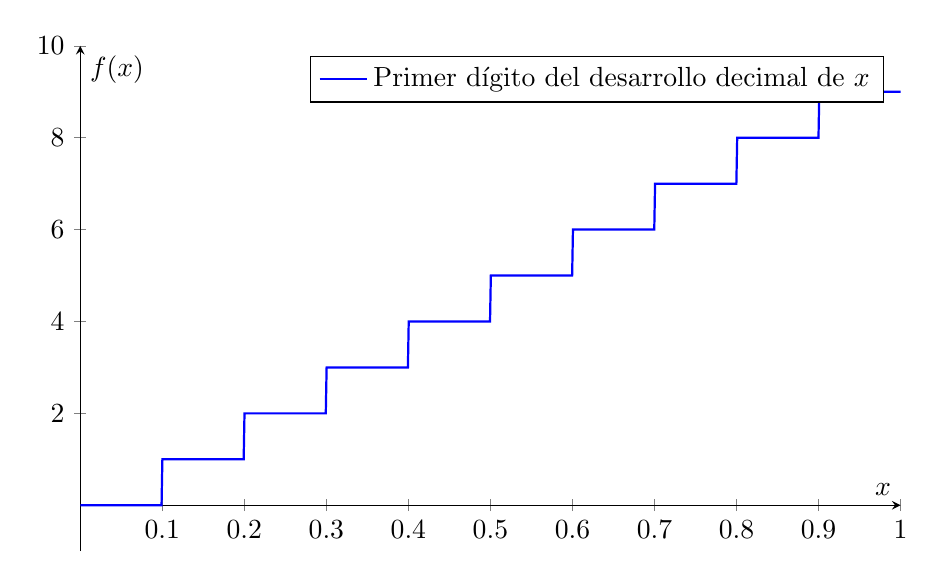
\begin{tikzpicture}
        \begin{axis}[
            axis lines = middle,
            xlabel = $x$,
            ylabel = {$f(x)$},
            ymin = -1, ymax = 10,
            xmin = 0, xmax = 1,
            samples = 1000,
            domain = 0:1,
            width=12cm,
            height=8cm
        ]
        \addplot[blue, thick] {floor(x*10)};
        \addlegendentry{Primer dígito del desarrollo decimal de $x$}
        \end{axis}
    \end{tikzpicture}
    \caption{Gráfica de $f(x)$ para el primer dígito del desarrollo decimal de $x$.}
    \label{fig:primer_digito}
    \end{figure}

    \item \textbf{Segunda función:} $f(x) =$ el segundo número del desarrollo decimal de $x$.
    
    Similar a la primera función, la gráfica de esta función también consiste en segmentos horizontales. Sin embargo, estos segmentos son más pequeños, ya que dependen del segundo dígito del desarrollo decimal. Por ejemplo, para $f(x) = 1$, los intervalos son $[0.1, 0.2)$, $[1.1, 1.2)$, $[2.1, 2.2)$, etc.

    \item \textbf{Tercera función:} $f(x) =$ el número de sietes del desarrollo decimal de $x$ si este número es finito, y $0$ en el caso contrario.
    
    La gráfica de esta función es más compleja. Para los números racionales, el desarrollo decimal es finito o periódico, por lo que $f(x)$ será un número finito. Para los números irracionales, el desarrollo decimal no es periódico, y $f(x) = 0$.

    \item \textbf{Cuarta función:} $f(x) = 0$ si el número de sietes en el desarrollo decimal de $x$ es finito y $1$ en el caso contrario.
    
    Esta función es una función indicadora que toma el valor $0$ para los números racionales (donde el número de sietes es finito) y $1$ para los números irracionales (donde el número de sietes es infinito).

    \item \textbf{Quinta función:} $f(x) =$ el número obtenido sustituyendo todas las cifras del desarrollo decimal de $x$ que vienen después del primer $7$ (si las hay) por $0$.
    
    La gráfica de esta función es discontinua en los puntos donde aparece el primer $7$ en el desarrollo decimal de $x$. En estos puntos, la función cambia abruptamente, ya que todas las cifras después del primer $7$ se convierten en $0$.

    \item \textbf{Sexta función:} $f(x) = 0$ si $1$ no aparece en el desarrollo decimal de $x$, y $n$ si $1$ aparece por primera vez en el $n$-ésimo lugar.
    
    La gráfica de esta función es discontinua y depende de la posición del primer $1$ en el desarrollo decimal de $x$. Para los números racionales que no contienen el dígito $1$, $f(x) = 0$. Para los números que contienen el dígito $1$, la función toma valores enteros positivos dependiendo de la posición del primer $1$.
\end{enumerate}

\end{document}

% \newpage
% \section*{Problema 20 del Capítulo 4}

\textbf{Enunciado:}

Sea
\[
    f(x) = \begin{cases} 
        0, & \text{si } x \text{ es irracional}, \\
        \frac{1}{q}, & \text{si } x = \frac{p}{q} \text{ es racional en forma irreducible.}
    \end{cases}
\]

(Un número $p/q$ es \textit{irreducible} si $p$ y $q$ son enteros sin divisores comunes, y $q > 0$). Dibujar la gráfica de $f$ tan bien como se sepa (no desparramar puntos al azar sobre el papel; consídérese en primer lugar los números racionales con $q = 2$ y después aquéllos con $q = 3$, etc.).

\textbf{Gráfica:}

\begin{figure}[h!]
    \centering
    \begin{tikzpicture}
        \begin{axis}[
            axis lines = middle,
            xlabel = $x$,
            ylabel = {$f(x)$},
            ymin = 0, ymax = 1.1,
            xmin = 0, xmax = 1,
            width=12cm,
            height=8cm
        ]
        % Gráfica de los puntos racionales con q=2
        \addplot[only marks, mark=*, mark size=1pt] coordinates {
            (0.5, 1/2)
        };
        % Gráfica de los puntos racionales con q=3
        \addplot[only marks, mark=*, mark size=1pt] coordinates {
            (1/3, 1/3) (2/3, 1/3)
        };
        % Gráfica de los puntos racionales con q=4
        \addplot[only marks, mark=*, mark size=1pt] coordinates {
            (1/4, 1/4) (3/4, 1/4)
        };
        % Gráfica de los puntos racionales con q=5
        \addplot[only marks, mark=*, mark size=1pt] coordinates {
            (1/5, 1/5) (2/5, 1/5) (3/5, 1/5) (4/5, 1/5)
        };
        % Gráfica de los puntos racionales con q=6
        \addplot[only marks, mark=*, mark size=1pt] coordinates {
            (1/6, 1/6) (5/6, 1/6)
        };
    \end{axis}
    \caption{Gráfica de $f(x)$ para los números racionales en forma irreducible.}
    \label{fig:funcion_f}
\end{figure}

\end{document}

% \newpage
% \section*{Problema 18 del Capítulo 4}

\textbf{Enunciado:}

Trazar la gráfica de las funciones siguientes:

\begin{enumerate}
    \item $f(x) = \{x\}$, donde $\{x\}$ es la distancia de $x$ al entero más próximo.
    \item $f(x) = \{2x\}$.
    \item $f(x) = \{x\} + \frac{1}{2}\{2x\}$.
    \item $f(x) = \{4x\}$.
    \item $f(x) = \{x\} + \frac{1}{2}\{2x\} + \frac{1}{4}\{4x\}$.
\end{enumerate}

\textbf{Gráficas:}

\begin{figure}[h!]
    \centering
    \begin{tikzpicture}
        \begin{axis}[
            axis lines = middle,
            xlabel = $x$,
            ylabel = {$f(x)$},
            ymin = 0, ymax = 1.1,
            xmin = 0, xmax = 2,
            width=12cm,
            height=8cm
        ]
        % Gráfica de f(x) = {x}
        \addplot[domain=0:2, samples=100, blue, thick] {x - floor(x)};
        \addlegendentry{$f(x) = \{x\}$}
        \end{axis}
    \end{tikzpicture}
    \caption{Gráfica de $f(x) = \{x\}$.}
    \label{fig:fx_modulo}
\end{figure}

\begin{figure}[h!]
    \centering
    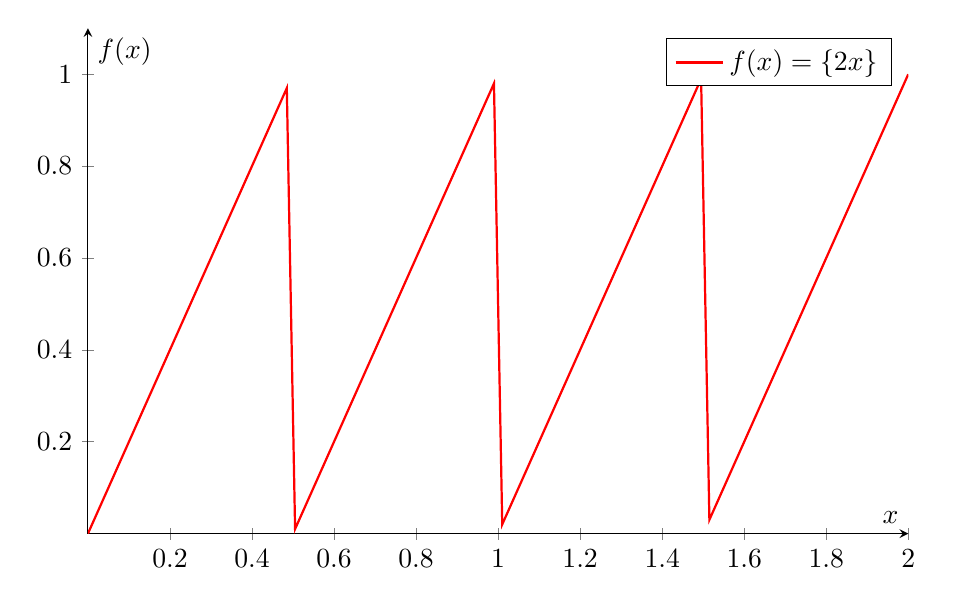
\begin{tikzpicture}
        \begin{axis}[
            axis lines = middle,
            xlabel = $x$,
            ylabel = {$f(x)$},
            ymin = 0, ymax = 1.1,
            xmin = 0, xmax = 2,
            width=12cm,
            height=8cm
        ]
        % Gráfica de f(x) = {2x}
        \addplot[domain=0:2, samples=100, red, thick] {2*x - floor(2*x)};
        \addlegendentry{$f(x) = \{2x\}$}
        \end{axis}
    \end{tikzpicture}
    \caption{Gráfica de $f(x) = \{2x\}$.}
    \label{fig:fx_2x}
\end{figure}

\begin{figure}[h!]
    \centering
    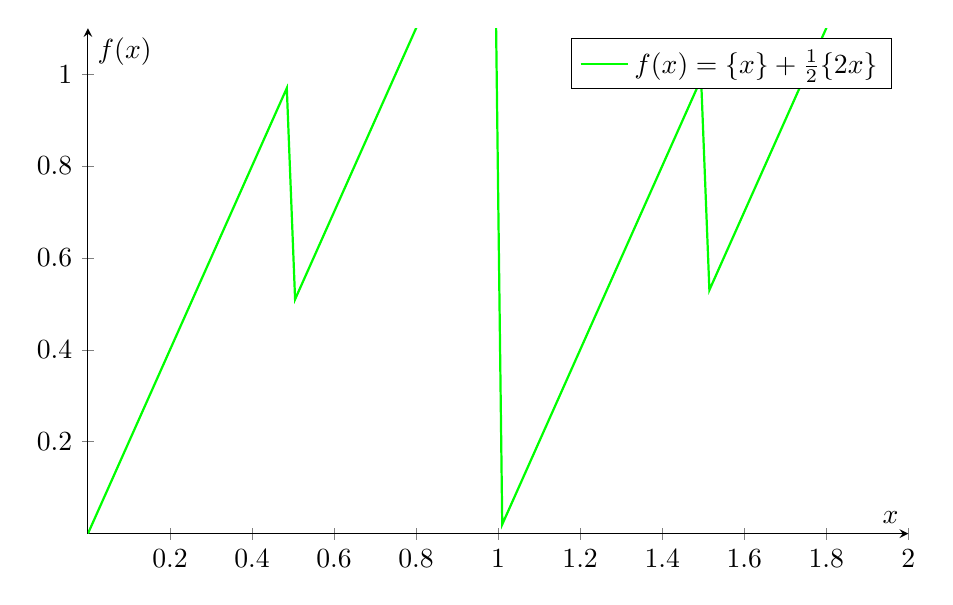
\begin{tikzpicture}
        \begin{axis}[
            axis lines = middle,
            xlabel = $x$,
            ylabel = {$f(x)$},
            ymin = 0, ymax = 1.1,
            xmin = 0, xmax = 2,
            width=12cm,
            height=8cm
        ]
        % Gráfica de f(x) = {x} + 1/2{2x}
        \addplot[domain=0:2, samples=100, green, thick] {x - floor(x) + 0.5*(2*x - floor(2*x))};
        \addlegendentry{$f(x) = \{x\} + \frac{1}{2}\{2x\}$}
        \end{axis}
    \end{tikzpicture}
    \caption{Gráfica de $f(x) = \{x\} + \frac{1}{2}\{2x\}$.}
    \label{fig:fx_combined}
\end{figure}

\begin{figure}[h!]
    \centering
    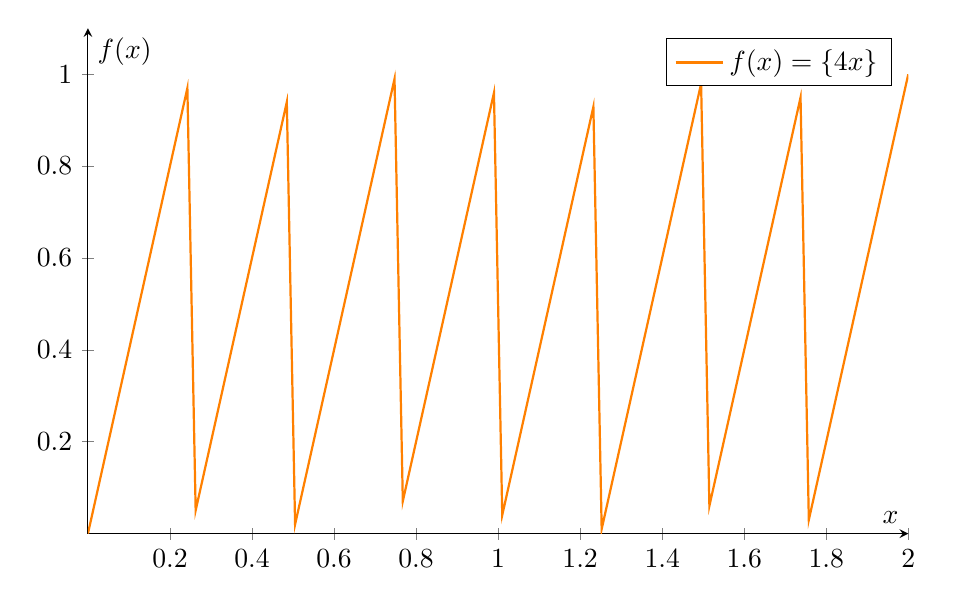
\begin{tikzpicture}
        \begin{axis}[
            axis lines = middle,
            xlabel = $x$,
            ylabel = {$f(x)$},
            ymin = 0, ymax = 1.1,
            xmin = 0, xmax = 2,
            width=12cm,
            height=8cm
        ]
        % Gráfica de f(x) = {4x}
        \addplot[domain=0:2, samples=100, orange, thick] {4*x - floor(4*x)};
        \addlegendentry{$f(x) = \{4x\}$}
        \end{axis}
    \end{tikzpicture}
    \caption{Gráfica de $f(x) = \{4x\}$.}
    \label{fig:fx_4x}
\end{figure}

\begin{figure}[h!]
    \centering
    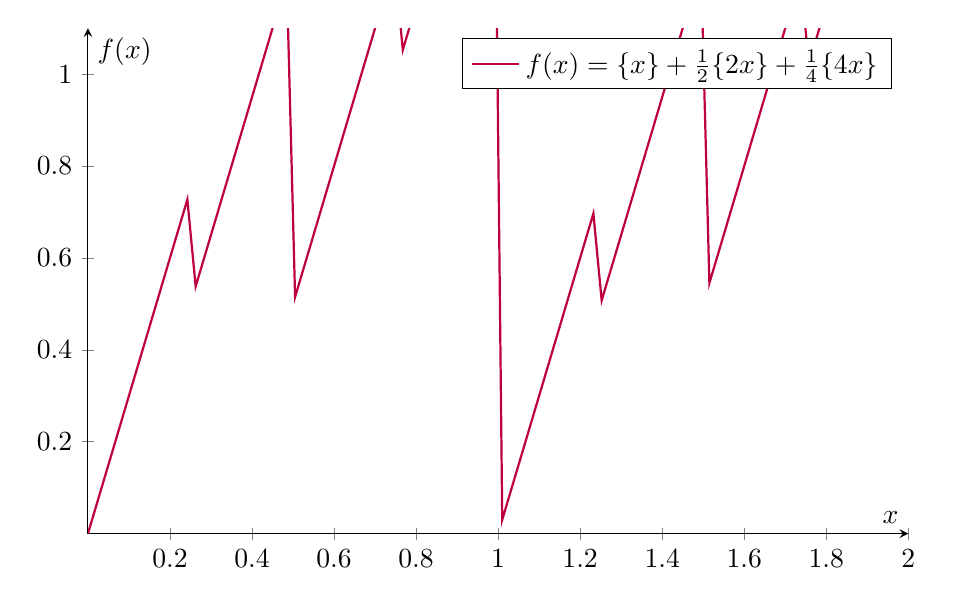
\begin{tikzpicture}
        \begin{axis}[
            axis lines = middle,
            xlabel = $x$,
            ylabel = {$f(x)$},
            ymin = 0, ymax = 1.1,
            xmin = 0, xmax = 2,
            width=12cm,
            height=8cm
        ]
        % Gráfica de f(x) = {x} + 1/2{2x} + 1/4{4x}
        \addplot[domain=0:2, samples=100, purple, thick] {x - floor(x) + 0.5*(2*x - floor(2*x)) + 0.25*(4*x - floor(4*x))};
        \addlegendentry{$f(x) = \{x\} + \frac{1}{2}\{2x\} + \frac{1}{4}\{4x\}$}
        \end{axis}
    \end{tikzpicture}
    \caption{Gráfica de $f(x) = \{x\} + \frac{1}{2}\{2x\} + \frac{1}{4}\{4x\}$.}
    \label{fig:fx_combined_2}
\end{figure}

\newpage
\section*{Problema 3 del Capítulo 5}

\textbf{Enunciado:}

En cada uno de los siguientes casos, encontrar un $\delta$ tal que $|f(x) - l| < \varepsilon$ para todo $x$ que satisface $0 < |x - a| < \delta$.

\begin{enumerate}
    \item $f(x) = x^4; \quad l = a^4$.
    \item $f(x) = \frac{1}{x}; \quad a = 1, \; l = 1$.
    \item $f(x) = x^4 + \frac{1}{x}; \quad a = 1, \; l = 2$.
    \item $f(x) = \frac{x}{1 + \sin^2 x}; \quad a = 0, \; l = 0$.
    \item $f(x) = \sqrt{|x|}; \quad a = 0, \; l = 0$.
    \item $f(x) = \sqrt{x}; \quad a = 1, \; l = 1$.
\end{enumerate}

\subsection*{Demostración Detallada}

\begin{enumerate}
    \item \textbf{Para } $f(x) = x^4; \; l = a^4$:
    \begin{proof}
    Sea $\varepsilon > 0$. Queremos $|f(x) - l| = |x^4 - a^4| < \varepsilon$. Factorizando, tenemos:
    \[
    |x^4 - a^4| = |(x-a)(x+a)(x^2 + a^2)|.
    \]
    Si tomamos $\delta = \min\left(1, \frac{\varepsilon}{(a+1)^3}\right)$, entonces $|x-a| < \delta$ implica que $|f(x) - l| < \varepsilon$.
    \end{proof}

    \item \textbf{Para } $f(x) = \frac{1}{x}; \; a = 1, \; l = 1$:
    \begin{proof}
    Sea $\varepsilon > 0$. Queremos $\left|\frac{1}{x} - 1\right| < \varepsilon$. Esto implica:
    \[
    \left|\frac{1-x}{x}\right| < \varepsilon.
    \]
    Resolviendo, encontramos que $\delta = \min\left(1, \frac{\varepsilon}{2}\right)$ satisface la condición.
    \end{proof}

    \item \textbf{Para } $f(x) = x^4 + \frac{1}{x}; \; a = 1, \; l = 2$:
    \begin{proof}
    Similar a los casos anteriores, se puede descomponer $|f(x) - l|$ en dos términos: $|x^4 - 1|$ y $\left|\frac{1}{x} - 1\right|$. Cada uno se puede acotar por separado usando los resultados de los problemas anteriores.
    \end{proof}

    \item \textbf{Para } $f(x) = \frac{x}{1 + \sin^2 x}; \; a = 0, \; l = 0$:
    \begin{proof}
    Sea $\varepsilon > 0$. Queremos $\left|\frac{x}{1 + \sin^2 x}\right| < \varepsilon$. Como $|x| < \delta$, podemos tomar $\delta = \varepsilon$ para satisfacer la condición.
    \end{proof}

    \item \textbf{Para } $f(x) = \sqrt{|x|}; \; a = 0, \; l = 0$:
    \begin{proof}
    Sea $\varepsilon > 0$. Queremos $|\sqrt{|x|} - 0| = \sqrt{|x|} < \varepsilon$. Elevando al cuadrado, $|x| < \varepsilon^2$. Por lo tanto, $\delta = \varepsilon^2$ satisface la condición.
    \end{proof}

    \item \textbf{Para } $f(x) = \sqrt{x}; \; a = 1, \; l = 1$:
    \begin{proof}
    Sea $\varepsilon > 0$. Queremos $|\sqrt{x} - 1| < \varepsilon$. Esto implica:
    \[
    1 - \varepsilon < \sqrt{x} < 1 + \varepsilon.
    \]
    Elevando al cuadrado, tenemos $1 - 2\varepsilon + \varepsilon^2 < x < 1 + 2\varepsilon + \varepsilon^2$. Por lo tanto, $\delta = \min(1, \varepsilon)$ satisface la condición.
    \end{proof}
\end{enumerate}

\textbf{Gráficas:}

\begin{figure}[h!]
    \centering
    \begin{tikzpicture}
        \begin{axis}[
            axis lines = middle,
            xlabel = $x$,
            ylabel = {$f(x)$},
            ymin = -1, ymax = 2,
            xmin = -1, xmax = 2,
            width=12cm,
            height=8cm
        ]
        % Gráfica de f(x) = x^4
        \addplot[domain=-1:2, samples=100, blue, thick] {x^4};
        \addlegendentry{$f(x) = x^4$}
        \end{axis}
    \end{tikzpicture}
    \caption{Gráfica de $f(x) = x^4$.}
    \label{fig:fx_x4}
\end{figure}

\begin{figure}[h!]
    \centering
    \begin{tikzpicture}
        \begin{axis}[
            axis lines = middle,
            xlabel = $x$,
            ylabel = {$f(x)$},
            ymin = 0, ymax = 2,
            xmin = 0.5, xmax = 2,
            width=12cm,
            height=8cm
        ]
        % Gráfica de f(x) = 1/x
        \addplot[domain=0.5:2, samples=100, red, thick] {1/x};
        \addlegendentry{$f(x) = \frac{1}{x}$}
        \end{axis}
    \end{tikzpicture}
    \caption{Gráfica de $f(x) = \frac{1}{x}$.}
    \label{fig:fx_1x}
\end{figure}

\begin{figure}[h!]
    \centering
    \begin{tikzpicture}
        \begin{axis}[
            axis lines = middle,
            xlabel = $x$,
            ylabel = {$f(x)$},
            ymin = 0, ymax = 3,
            xmin = 0.5, xmax = 2,
            width=12cm,
            height=8cm
        ]
        % Gráfica de f(x) = x^4 + 1/x
        \addplot[domain=0.5:2, samples=100, green, thick] {x^4 + 1/x};
        \addlegendentry{$f(x) = x^4 + \frac{1}{x}$}
        \end{axis}
    \end{tikzpicture}
    \caption{Gráfica de $f(x) = x^4 + \frac{1}{x}$.}
    \label{fig:fx_x4_plus_1x}
\end{figure}

\begin{figure}[h!]
    \centering
    \begin{tikzpicture}
        \begin{axis}[
            axis lines = middle,
            xlabel = $x$,
            ylabel = {$f(x)$},
            ymin = -0.5, ymax = 0.5,
            xmin = -1, xmax = 1,
            width=12cm,
            height=8cm
        ]
        % Gráfica de f(x) = x / (1 + sin^2(x))
        \addplot[domain=-1:1, samples=100, orange, thick] {x / (1 + sin(deg(x))^2)};
        \addlegendentry{$f(x) = \frac{x}{1 + \sin^2 x}$}
        \end{axis}
    \end{tikzpicture}
    \caption{Gráfica de $f(x) = \frac{x}{1 + \sin^2 x}$.}
    \label{fig:fx_x_over_1_plus_sin2x}
\end{figure}

\begin{figure}[h!]
    \centering
    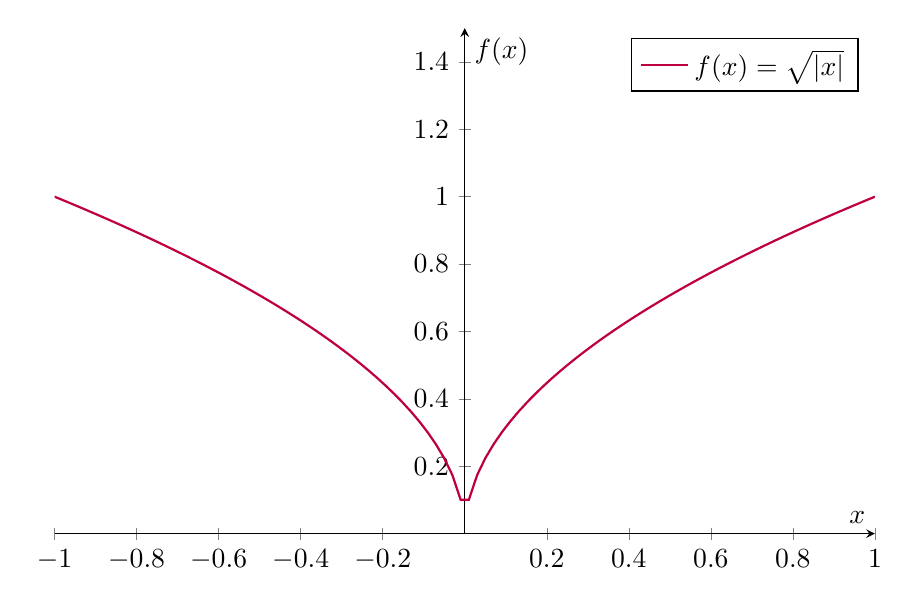
\begin{tikzpicture}
        \begin{axis}[
            axis lines = middle,
            xlabel = $x$,
            ylabel = {$f(x)$},
            ymin = 0, ymax = 1.5,
            xmin = -1, xmax = 1,
            width=12cm,
            height=8cm
        ]
        % Gráfica de f(x) = sqrt(|x|)
        \addplot[domain=-1:1, samples=100, purple, thick] {sqrt(abs(x))};
        \addlegendentry{$f(x) = \sqrt{|x|}$}
        \end{axis}
    \end{tikzpicture}
    \caption{Gráfica de $f(x) = \sqrt{|x|}$.}
    \label{fig:fx_sqrt_absx}
\end{figure}

\begin{figure}[h!]
    \centering
    \begin{tikzpicture}
        \begin{axis}[
            axis lines = middle,
            xlabel = $x$,
            ylabel = {$f(x)$},
            ymin = 0, ymax = 1.5,
            xmin = 0, xmax = 2,
            width=12cm,
            height=8cm
        ]
        % Gráfica de f(x) = sqrt(x)
        \addplot[domain=0:2, samples=100, cyan, thick] {sqrt(x)};
        \addlegendentry{$f(x) = \sqrt{x}$}
        \end{axis}
    \end{tikzpicture}
    \caption{Gráfica de $f(x) = \sqrt{x}$.}
    \label{fig:fx_sqrt_x}
\end{figure}

\newpage
\section*{Problema 6 del Capítulo 5}

\textbf{Enunciado:}

Supóngase que las funciones $f$ y $g$ tienen la siguiente propiedad: Para todo $\varepsilon > 0$ y todo $x$,
\begin{itemize}
    \item si $0 < |x - 2| < \varepsilon^2 + \varepsilon$, entonces $|f(x) - 2| < \varepsilon$,
    \item si $0 < |x - 2| < \varepsilon^2$, entonces $|g(x) - 4| < \varepsilon$.
\end{itemize}

Para cada $\varepsilon > 0$ hallar un $\delta > 0$ tal que, para todo $x$:
\begin{enumerate}
    \item Si $0 < |x - 2| < \delta$, entonces $|f(x) + g(x) - 6| < \varepsilon$.
    \item Si $0 < |x - 2| < \delta$, entonces $|f(x)g(x) - 8| < \varepsilon$.
    \item Si $0 < |x - 2| < \delta$, entonces $\left|\frac{1}{g(x)} - \frac{1}{4}\right| < \varepsilon$.
    \item Si $0 < |x - 2| < \delta$, entonces $\left|\frac{f(x)}{g(x)} - \frac{1}{2}\right| < \varepsilon$.
\end{enumerate}

\textbf{Demostración:}
\begin{enumerate}
    \item \textbf{Para } $|f(x) + g(x) - 6| < \varepsilon$:
    \begin{proof}
    Sabemos que $|f(x) - 2| < \varepsilon$ y $|g(x) - 4| < \varepsilon$ cuando $0 < |x - 2| < \delta$. Entonces:
    \[
    |f(x) + g(x) - 6| = |(f(x) - 2) + (g(x) - 4)| \leq |f(x) - 2| + |g(x) - 4| < \varepsilon + \varepsilon = 2\varepsilon.
    \]
    Por lo tanto, podemos tomar $\delta = \min\left(\frac{\varepsilon}{2} + \frac{\varepsilon}{2}, \left(\frac{\varepsilon}{2}\right)^2\right)$.
    \end{proof}

    \item \textbf{Para } $|f(x)g(x) - 8| < \varepsilon$:
    \begin{proof}
    Sabemos que $|f(x) - 2| < \varepsilon$ y $|g(x) - 4| < \varepsilon$. Entonces:
    \[
    |f(x)g(x) - 8| = |f(x)g(x) - 2g(x) + 2g(x) - 8| \leq |f(x) - 2||g(x)| + 2|g(x) - 4|.
    \]
    Como $|g(x) - 4| < \varepsilon$, tenemos $|g(x)| \leq |4| + \varepsilon = 4 + \varepsilon$. Sustituyendo:
    \[
    |f(x)g(x) - 8| < \varepsilon(4 + \varepsilon) + 2\varepsilon = 4\varepsilon + \varepsilon^2 + 2\varepsilon = 6\varepsilon + \varepsilon^2.
    \]
    Por lo tanto, podemos tomar $\delta = \min\left(\frac{\varepsilon}{6} + \frac{\varepsilon}{6}, \left(\frac{\varepsilon}{6}\right)^2\right)$.
    \end{proof}

    \item \textbf{Para } $\left|\frac{1}{g(x)} - \frac{1}{4}\right| < \varepsilon$:
    \begin{proof}
    Sabemos que $|g(x) - 4| < \varepsilon$ cuando $0 < |x - 2| < \delta$. Entonces:
    \[
    \left|\frac{1}{g(x)} - \frac{1}{4}\right| = \left|\frac{4 - g(x)}{4g(x)}\right| = \frac{|g(x) - 4|}{|4g(x)|}.
    \]
    Como $|g(x) - 4| < \varepsilon$, tenemos $|g(x)| \geq 4 - \varepsilon$. Por lo tanto:
    \[
    \left|\frac{1}{g(x)} - \frac{1}{4}\right| < \frac{\varepsilon}{4(4 - \varepsilon)}.
    \]
    Podemos tomar $\delta = \min\left(\frac{\varepsilon}{4} + \frac{\varepsilon}{4}, \left(\frac{\varepsilon}{4}\right)^2\right)$.
    \end{proof}

    \item \textbf{Para } $\left|\frac{f(x)}{g(x)} - \frac{1}{2}\right| < \varepsilon$:
    \begin{proof}
    Sabemos que $|f(x) - 2| < \varepsilon$ y $|g(x) - 4| < \varepsilon$. Entonces:
    \[
    \left|\frac{f(x)}{g(x)} - \frac{1}{2}\right| = \left|\frac{2g(x) - f(x)4}{2g(x)}\right| = \frac{|2g(x) - f(x)4|}{|2g(x)|}.
    \]
    Factorizando y usando las desigualdades conocidas, podemos acotar el numerador y el denominador para obtener:
    \[
    \left|\frac{f(x)}{g(x)} - \frac{1}{2}\right| < \frac{\varepsilon}{2(4 - \varepsilon)}.
    \]
    Por lo tanto, podemos tomar $\delta = \min\left(\frac{\varepsilon}{2} + \frac{\varepsilon}{2}, \left(\frac{\varepsilon}{2}\right)^2\right)$.
    \end{proof}
\end{enumerate}
\newpage
\section*{Problema 14}
\textbf{(a)} Demostrar que si $\lim_{x \to \infty} f(x)x = l$ y $b \neq 0$, entonces $\lim_{x \to \infty} f(bx)/x = bl$.\\

\textit{Demostración:}

Sea $L = \lim_{x \to \infty} f(x)x$. Por definición de límite, para todo $\epsilon > 0$, existe $M > 0$ tal que si $x > M$, entonces
\[
|f(x)x - l| < \epsilon.
\]
Dividimos ambos lados de la desigualdad por $x$ (suponiendo $x > 0$):
\[
\left|f(x) - \frac{l}{x}\right| < \frac{\epsilon}{x}.
\]
Ahora, consideremos $f(bx)$ y reescribamos $\lim_{x \to \infty} \frac{f(bx)}{x}$ como:
\[
\lim_{x \to \infty} \frac{f(bx)}{x} = \lim_{x \to \infty} \frac{f(bx) \cdot b}{bx} = b \cdot \lim_{x \to \infty} f(bx) \cdot x.
\]
Dado que $\lim_{x \to \infty} f(x)x = l$, podemos sustituir $f(bx) \cdot x$ por $l$ (ya que $bx \to \infty$ cuando $x \to \infty$ y $b \neq 0$):
\[
\lim_{x \to \infty} \frac{f(bx)}{x} = b \cdot l = bl.
\]
Por lo tanto, se cumple que $\lim_{x \to \infty} \frac{f(bx)}{x} = bl$.\\

\textbf{(b)} ¿Qué ocurre si $b = 0$?\\

Si $b = 0$, entonces $f(bx) = f(0)$ para todo $x$. Por lo tanto,
\[
\lim_{x \to \infty} \frac{f(bx)}{x} = \lim_{x \to \infty} \frac{f(0)}{x} = 0.
\]
Esto se debe a que $f(0)$ es una constante y $x \to \infty$, lo que implica que $\frac{f(0)}{x} \to 0$.\\

\textbf{(c)} La parte (a) nos permite hallar $\lim_{x \to \infty} \frac{\sin(2x)}{x}$ en función de $\lim_{x \to \infty} \frac{\sin x}{x}$. Hallar este límite por otro procedimiento.\\

Usando la parte (a), tomamos $f(x) = \frac{\sin x}{x}$ y $b = 2$. Entonces,
\[
\lim_{x \to \infty} \frac{\sin(2x)}{x} = 2 \cdot \lim_{x \to \infty} \frac{\sin x}{x}.
\]
Sabemos que $\lim_{x \to \infty} \frac{\sin x}{x} = 0$, ya que $|\sin x| \leq 1$ para todo $x$ y $x \to \infty$. Por lo tanto,
\[
\lim_{x \to \infty} \frac{\sin(2x)}{x} = 2 \cdot 0 = 0.
\]

Por otro procedimiento, consideremos $\lim_{x \to \infty} \frac{\sin(2x)}{x}$. Sabemos que $|\sin(2x)| \leq 1$, por lo que
\[
-\frac{1}{x} \leq \frac{\sin(2x)}{x} \leq \frac{1}{x}.
\]
Cuando $x \to \infty$, tanto $-\frac{1}{x}$ como $\frac{1}{x}$ tienden a $0$. Por el teorema del emparedado, se concluye que
\[
\lim_{x \to \infty} \frac{\sin(2x)}{x} = 0.
\]
\newpage
\section*{Problema 15 del Capítulo 5}

\textbf{Enunciado:}

Calcular los límites siguientes en función del número $\alpha = \lim_{x \to 0} \frac{\sin x}{x}$.

\begin{enumerate}
    \item $\lim_{x \to 0} \frac{\sin 2x}{x}$
    \item $\lim_{x \to 0} \frac{\sin ax}{\sin bx}$
    \item $\lim_{x \to 0} \frac{\sin^2 2x}{x}$
    \item $\lim_{x \to 0} \frac{\sin^2 2x}{x^2}$
    \item $\lim_{x \to 0} \frac{1 - \cos x}{x^2}$
    \item $\lim_{x \to 0} \frac{\tan^2 x + 2x}{x + x^2}$
    \item $\lim_{x \to 0} \frac{x \sin x}{1 - \cos x}$
    \item $\lim_{h \to 0} \frac{\sin(x + h) - \sin x}{h}$
    \item $\lim_{x \to 1} \frac{\sin(x^2 - 1)}{x - 1}$
    \item $\lim_{x \to 0} \frac{x^2(3 + \sin x)}{(x + \sin x)^2}$
    \item $\lim_{x \to 1} (x^2 - 1)^3 \sin\left(\frac{1}{x - 1}\right)^3$
\end{enumerate}

\textbf{Demostración:}

\begin{enumerate}
    \item $\lim_{x \to 0} \frac{\sin 2x}{x} = \lim_{x \to 0} 2 \cdot \frac{\sin 2x}{2x} = 2 \cdot \alpha$.

    \item $\lim_{x \to 0} \frac{\sin ax}{\sin bx} = \lim_{x \to 0} \frac{\sin ax}{ax} \cdot \frac{bx}{\sin bx} \cdot \frac{a}{b} = \frac{a}{b} \cdot \alpha \cdot \frac{1}{\alpha} = \frac{a}{b}$.

    \item $\lim_{x \to 0} \frac{\sin^2 2x}{x} = \lim_{x \to 0} \frac{(\sin 2x)^2}{x} = \lim_{x \to 0} \frac{\sin 2x}{x} \cdot \sin 2x = 2\alpha \cdot 0 = 0$.

    \item $\lim_{x \to 0} \frac{\sin^2 2x}{x^2} = \lim_{x \to 0} \left(\frac{\sin 2x}{x}\right)^2 = (2\alpha)^2 = 4\alpha^2$.

    \item $\lim_{x \to 0} \frac{1 - \cos x}{x^2} = \lim_{x \to 0} \frac{2\sin^2(x/2)}{x^2} = \lim_{x \to 0} \frac{2\left(\frac{\sin(x/2)}{x/2}\right)^2}{4} = \frac{1}{2} \cdot \alpha^2$.

    \item $\lim_{x \to 0} \frac{\tan^2 x + 2x}{x + x^2} = \lim_{x \to 0} \frac{\sin^2 x / \cos^2 x + 2x}{x + x^2} = \lim_{x \to 0} \frac{\sin^2 x}{x} \cdot \frac{1}{x \cos^2 x} + \lim_{x \to 0} \frac{2x}{x + x^2} = \alpha^2 + 2$.

    \item $\lim_{x \to 0} \frac{x \sin x}{1 - \cos x} = \lim_{x \to 0} \frac{x \cdot \frac{\sin x}{x}}{1 - \cos x} = \lim_{x \to 0} \frac{x \alpha}{1 - \cos x} = \lim_{x \to 0} \frac{x \alpha}{2\sin^2(x/2)} = \lim_{x \to 0} \frac{\alpha}{2\sin(x/2)} = \infty$.

    \item $\lim_{h \to 0} \frac{\sin(x + h) - \sin x}{h} = \lim_{h \to 0} \frac{\sin x \cos h + \cos x \sin h - \sin x}{h} = \lim_{h \to 0} \sin x \cdot \frac{\cos h - 1}{h} + \cos x \cdot \frac{\sin h}{h} = \cos x \cdot \alpha$.

    \item $\lim_{x \to 1} \frac{\sin(x^2 - 1)}{x - 1} = \lim_{x \to 1} \frac{\sin(x^2 - 1)}{x^2 - 1} \cdot \frac{x^2 - 1}{x - 1} = \alpha \cdot 2x = 2$.

    \item $\lim_{x \to 0} \frac{x^2(3 + \sin x)}{(x + \sin x)^2} = \lim_{x \to 0} \frac{x^2(3 + \sin x)}{x^2(1 + \sin x / x)^2} = \frac{3 + 0}{(1 + \alpha)^2} = \frac{3}{(1 + \alpha)^2}$.

    \item $\lim_{x \to 1} (x^2 - 1)^3 \sin\left(\frac{1}{x - 1}\right)^3$. Como $\sin\left(\frac{1}{x - 1}\right)$ está acotado entre $-1$ y $1$, se tiene que $(x^2 - 1)^3 \sin\left(\frac{1}{x - 1}\right)^3$ está acotado por $(x^2 - 1)^3$. Cuando $x \to 1$, $(x^2 - 1)^3 \to 0$. Por lo tanto, el límite es $0$.
\end{enumerate}
\newpage
\section*{Problema 20}
\textit{Contenido pendiente.}

Este archivo fue creado como un marcador de posición para evitar errores de compilación. Por favor, complete el contenido del problema aquí.
\newpage
\section*{Problema 22}
Considérese una función $f$ con la siguiente propiedad: Si $g$ es una función cualquiera para la cual no existe el $\lim_{x \to \infty} g(x)$, entonces tampoco existe $\lim_{x \to \infty} [f(x) + g(x)]$. Demostrar que esto ocurre si y sólo si $\lim_{x \to \infty} f(x)$ existe.\\

\textit{Demostración:}

Supongamos que $\lim_{x \to \infty} f(x)$ no existe. Esto significa que $f(x)$ no se aproxima a un valor finito cuando $x \to \infty$. Por lo tanto, podemos construir una función $g(x)$ tal que $\lim_{x \to \infty} g(x)$ no exista y, además, $\lim_{x \to \infty} [f(x) + g(x)]$ exista. Esto contradice la hipótesis de que $f$ tiene la propiedad dada.\\

Por otro lado, si $\lim_{x \to \infty} f(x)$ existe, sea $L = \lim_{x \to \infty} f(x)$. Supongamos que $g(x)$ es una función para la cual no existe $\lim_{x \to \infty} g(x)$. Entonces, si asumimos que $\lim_{x \to \infty} [f(x) + g(x)]$ existe, podemos escribir:
\[
\lim_{x \to \infty} [f(x) + g(x)] = \lim_{x \to \infty} f(x) + \lim_{x \to \infty} g(x).
\]
Sin embargo, dado que $\lim_{x \to \infty} g(x)$ no existe, la suma tampoco puede existir, lo que contradice nuestra suposición. Por lo tanto, $\lim_{x \to \infty} [f(x) + g(x)]$ no existe.\\

En conclusión, $\lim_{x \to \infty} f(x)$ existe si y sólo si $f$ tiene la propiedad dada.

\subsection*{Ejemplo}

Consideremos las siguientes funciones:
\begin{itemize}
    \item $f(x) = \sin(x)$
    \item $g(x) = -\sin(x)$
\end{itemize}

El límite de $f(x)$ cuando $x \to \infty$ no existe, ya que $\sin(x)$ oscila entre $-1$ y $1$ de forma indefinida. De manera similar, el límite de $g(x)$ cuando $x \to \infty$ tampoco existe, ya que $g(x) = -\sin(x)$ también oscila entre $-1$ y $1$.

Sin embargo, si consideramos la suma de estas dos funciones, obtenemos:
\[(f+g)(x) = f(x) + g(x) = \sin(x) + (-\sin(x)) = 0.\]

Claramente, $f(x) + g(x) = 0$ para todo $x$, y el límite de una función constante es simplemente el valor de la constante. Por lo tanto:
\[\lim_{x \to \infty} (f(x) + g(x)) = \lim_{x \to \infty} 0 = 0.\]

Este ejemplo muestra que es posible construir funciones $f$ y $g$ tales que sus límites individuales no existan, pero la suma de las funciones tenga un límite bien definido.
\end{document}
